\documentclass[envcountsect,dvips]{beamer}

\setbeamertemplate{background canvas}[vertical shading][bottom=yellow!20,top=blue!10]
%\usetheme{Darmstadt}
\usetheme{Warsaw}
%\usefonttheme[onlysmall]{structurebold}

\usepackage{natbib}
\usepackage{bibentry}
\bibliographystyle{apalike}
\usepackage{chngcntr}

\usepackage[utf8]{inputenc}
\usepackage{default}
\usepackage{amsmath}
\usepackage{amsfonts}
\usepackage{amssymb}

\usepackage{graphicx}
\usepackage{caption}
\usepackage{subcaption}

\usepackage{color,xcolor,ucs}% para textcolor



%%%%%%%%%%%%%%%%%%%%%%%%%%%%%%%%%%%%%%%%%%%%%%%%%%%%%%%%%%%%%%%%%%%%%%%%%%
\begin{document}

\title[Diodos semicondutores:  ] % (optional, only for long titles)
{Diodos semicondutores:}
\subtitle{Construção, caraterísticas e aplicações}
\author[Fernando] % (optional, for multiple authors)
{Fernando Pujaico Rivera\inst{1}}
\institute[Universidade Federal de Lavras] % (optional)
{
  \inst{1}%
  Universidade Federal de Lavras
}
\date[2016] % (optional)
{Aula-1 2016}
\subject{Computer Science}
\frame{\titlepage}

%%%%%%%%%%%%%%%%%%%%%%%%%%%%%%%%%%%%%%%%%%%%%%%%%%%%%%%%%%%%%%%%%%%%%%%%%%%%%%%%
%%%%%%%%%%%%%%%%%%%%%%%%%%%%%%%%%%%%%%%%%%%%%%%%%%%%%%%%%%%%%%%%%%%%%%%%%%%%%%%%
%%%%%%%%%%%%%%%%%%%%%%%%%%%%%%%%%%%%%%%%%%%%%%%%%%%%%%%%%%%%%%%%%%%%%%%%%%%%%%%%
\section{Construção }
%%https://www.youtube.com/watch?v=X0XscX9ugp0

\begin{frame}{Descrição simples do Diodo \cite{boylestaddispositivos} }
\begin{figure}
\centering
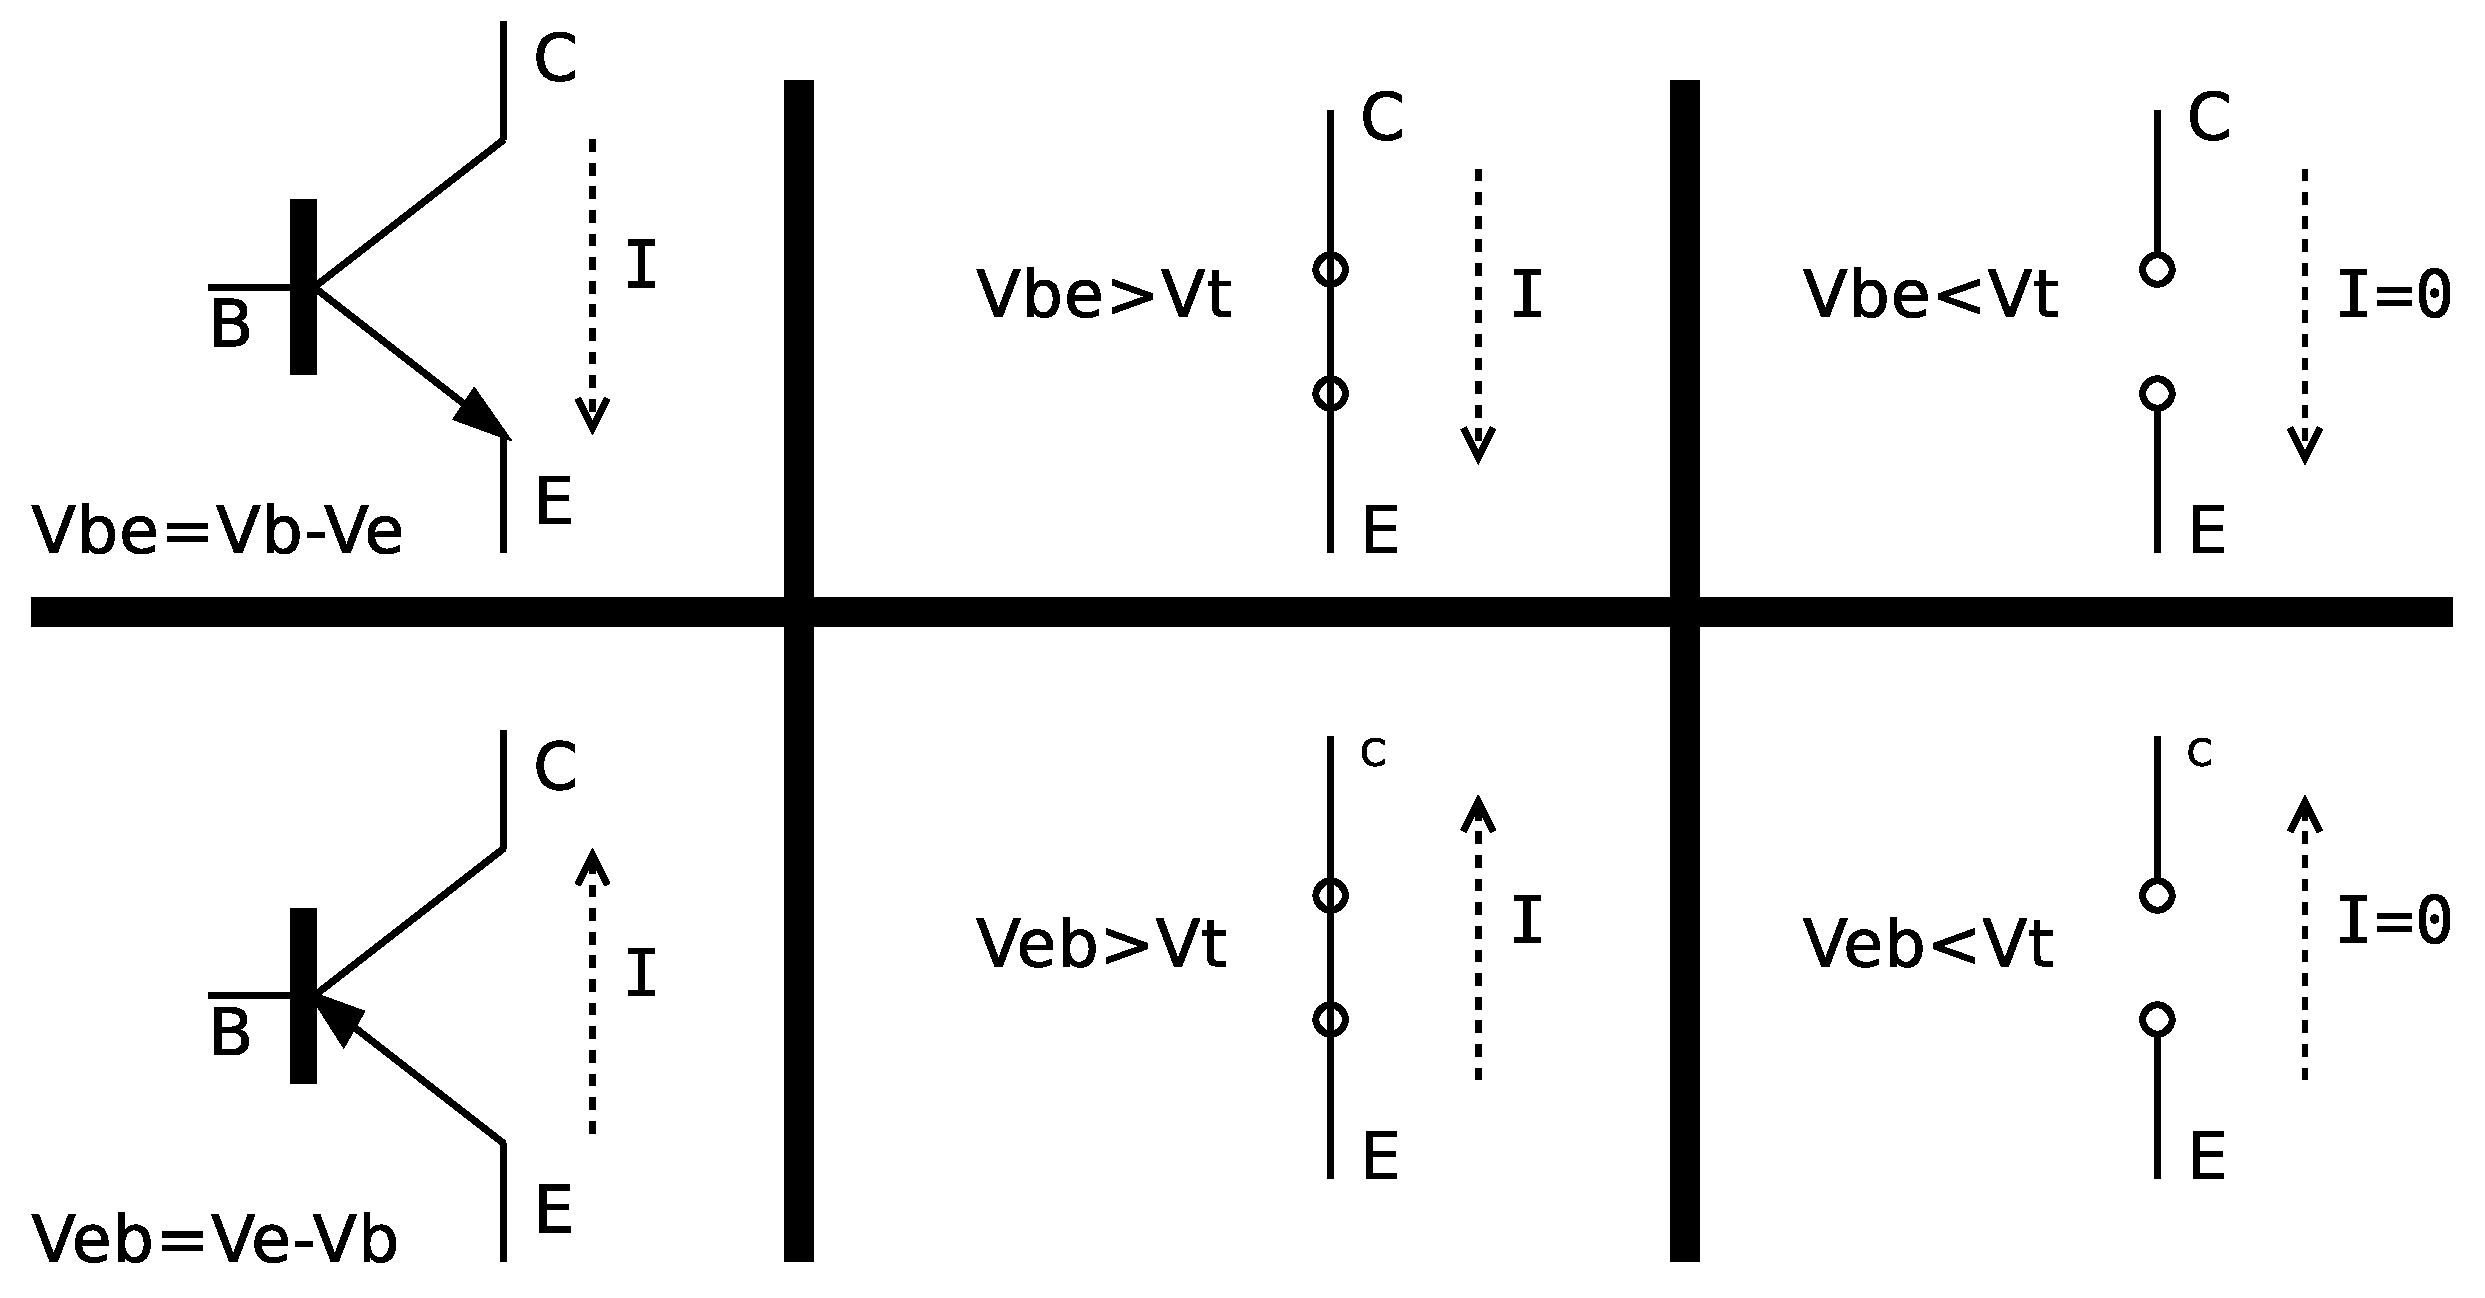
\includegraphics[width=9cm]{images/simple.eps}
\caption{Descrição simples do Diodo}
\label{fig:simples}
\end{figure}
\end{frame}


\begin{frame}{Semicondutor  }
\begin{figure}
\centering
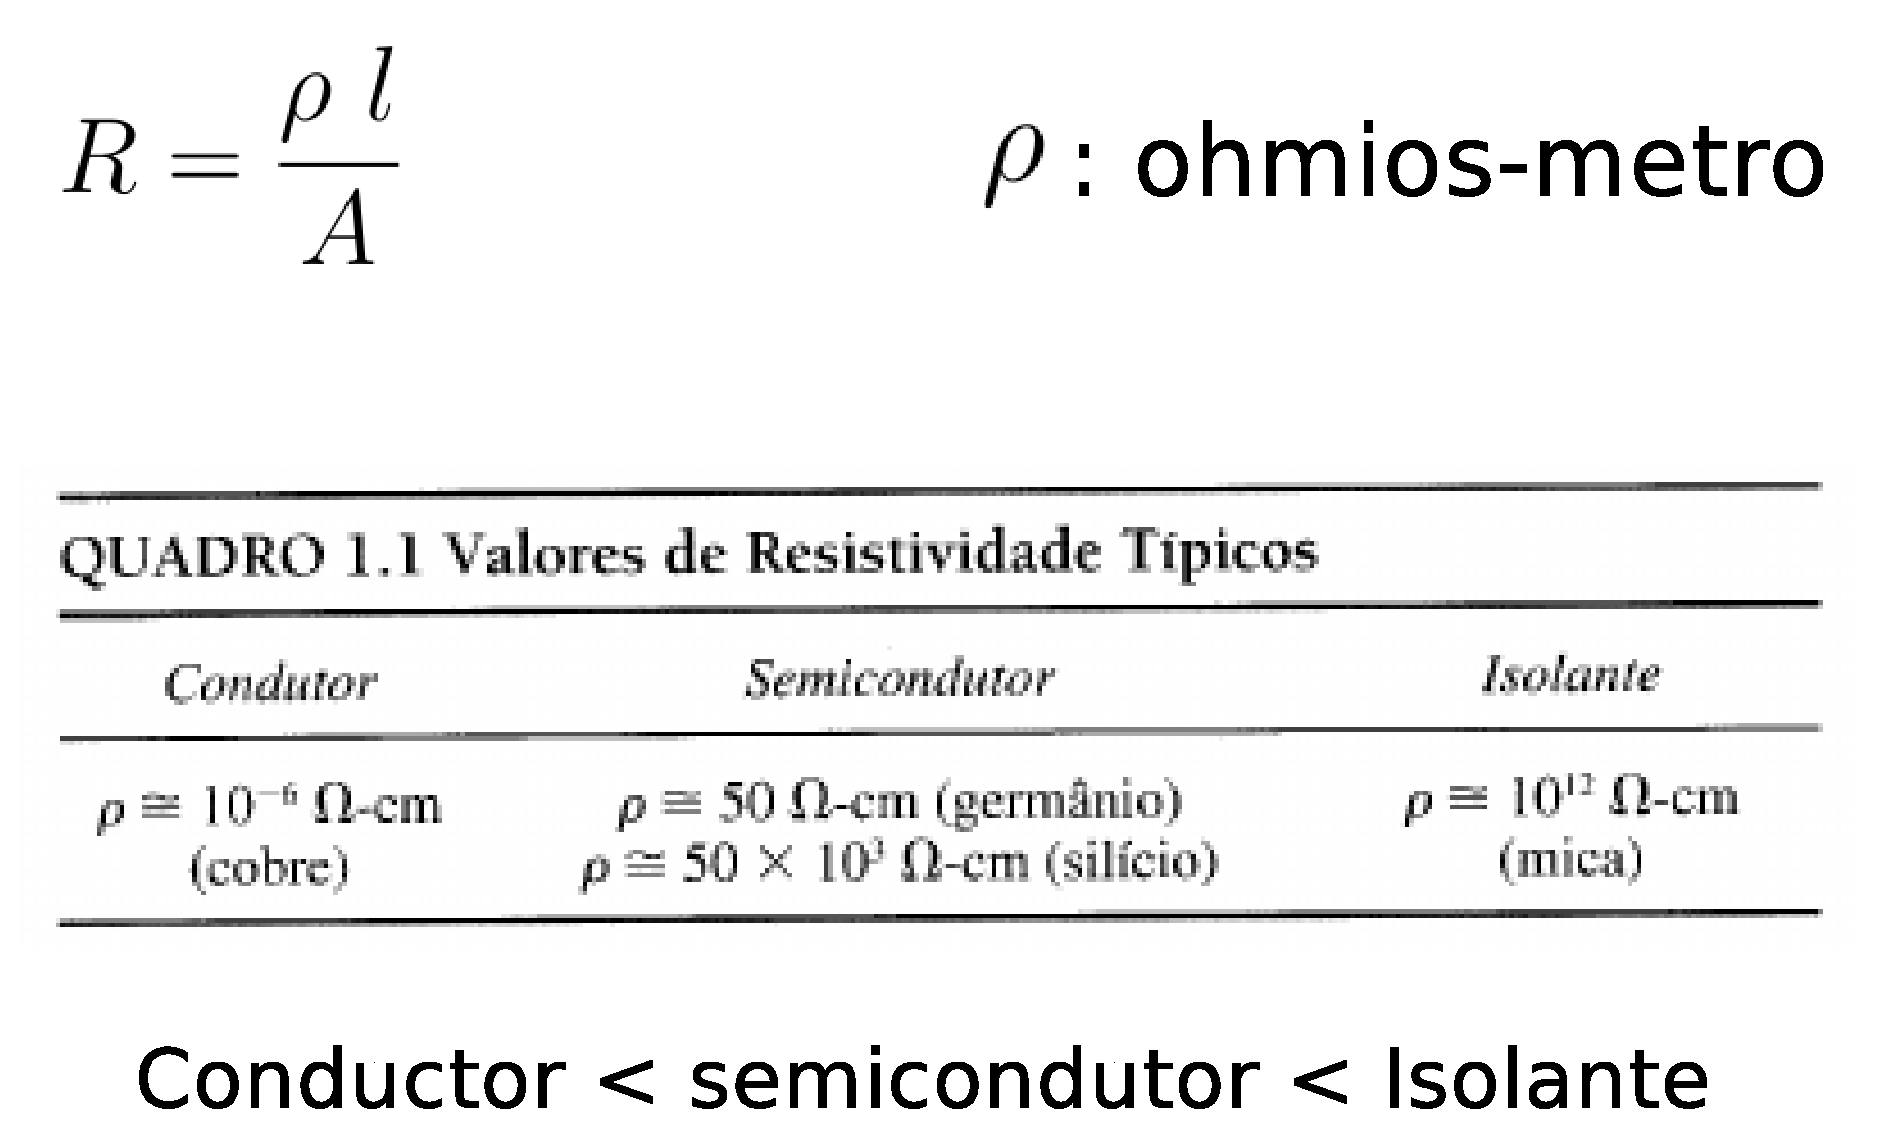
\includegraphics[width=9cm]{images/conductor.eps}
\caption{Resistência ao fluxo de carga}
\label{fig:conductor}
\end{figure}
\end{frame}

\begin{frame}{Materiais condutores   }
\begin{figure}
\centering
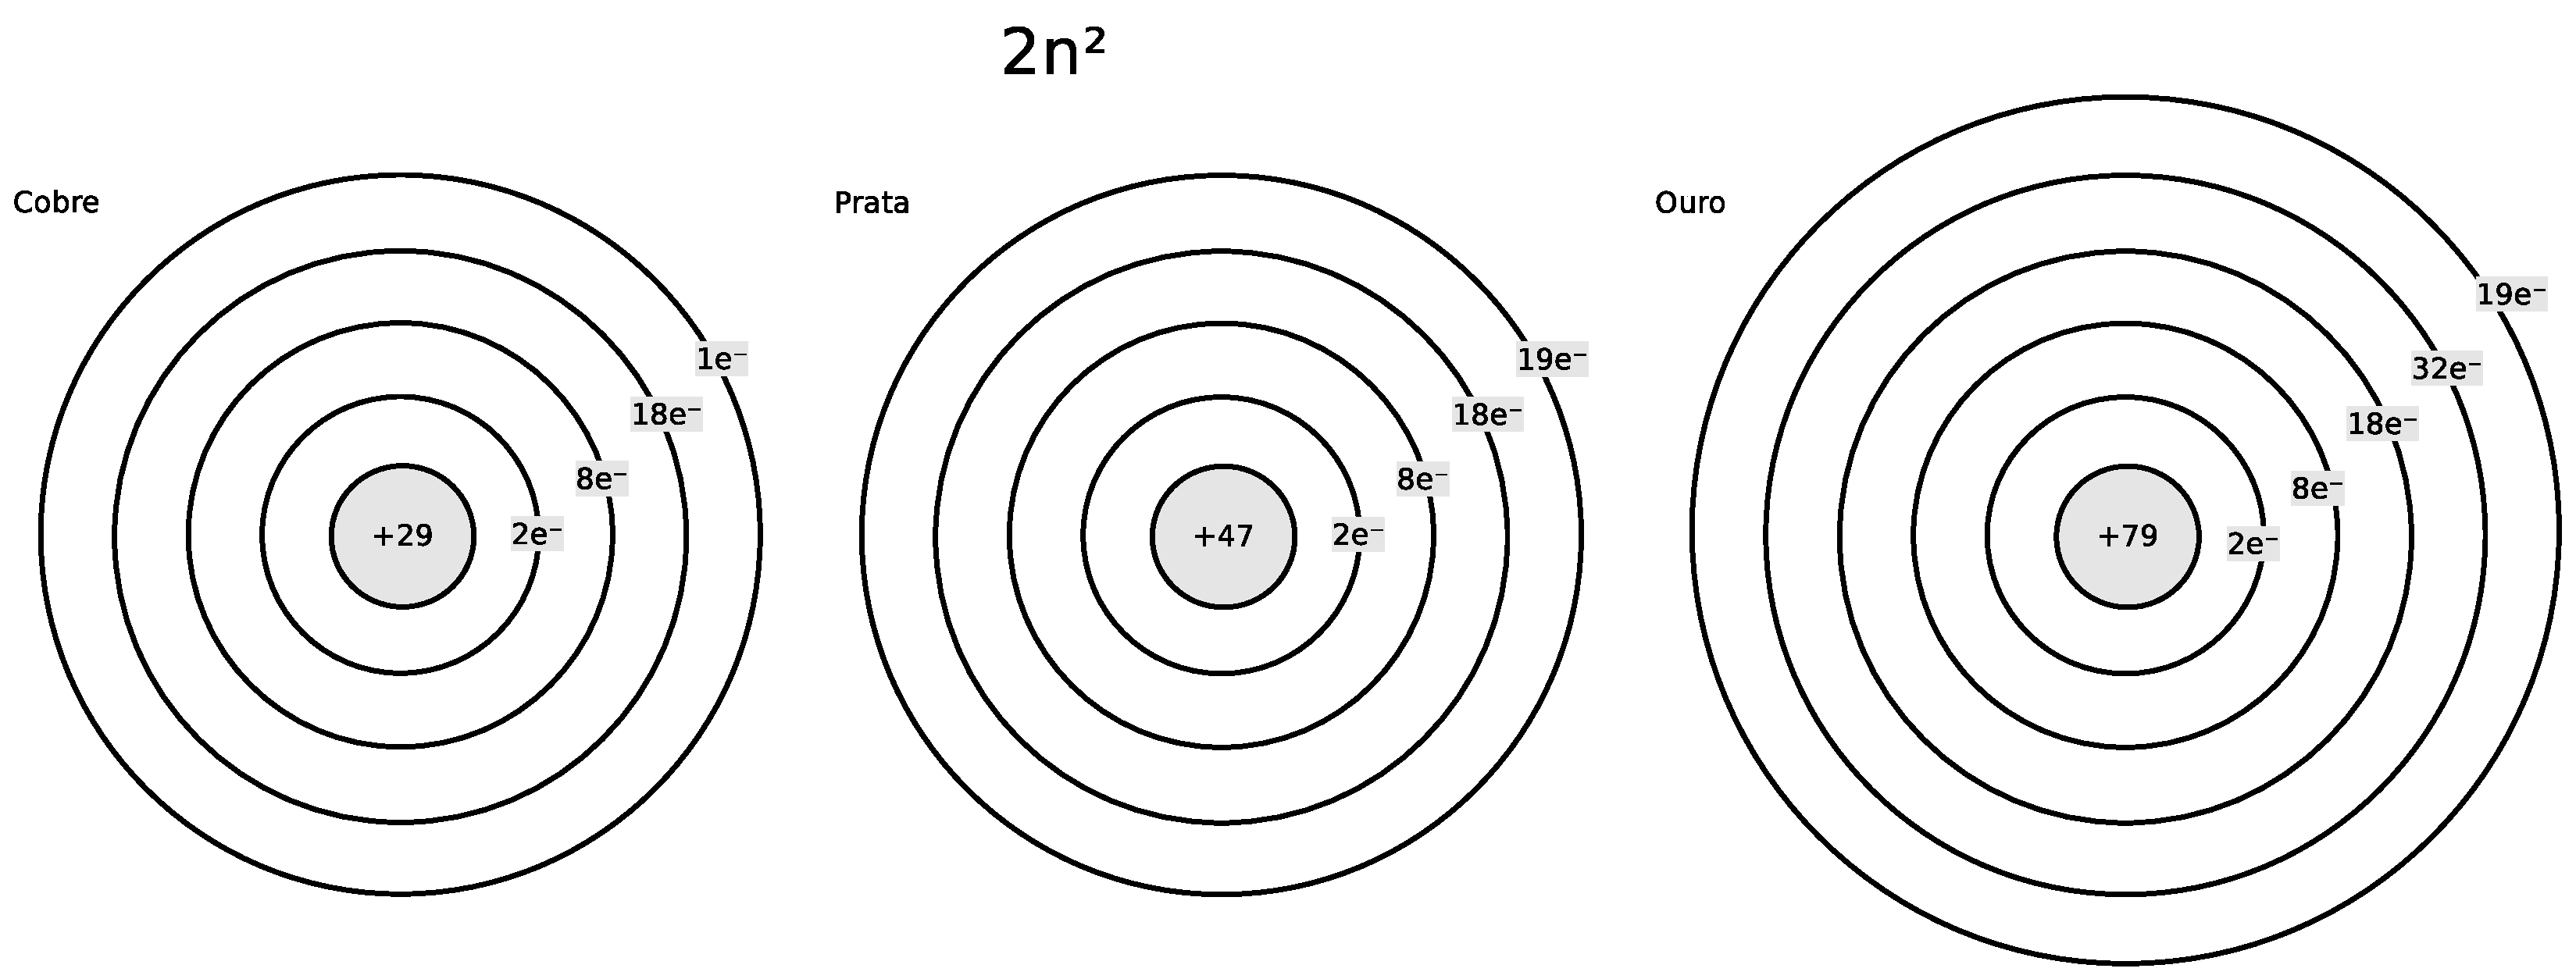
\includegraphics[width=10cm]{images/cobre.eps}
\caption{Elétrons nas camadas e camadas de valência}
\label{fig:dopagem}
\end{figure}
\end{frame}

\begin{frame}{Materiais semicondutores}
\begin{figure}
\centering
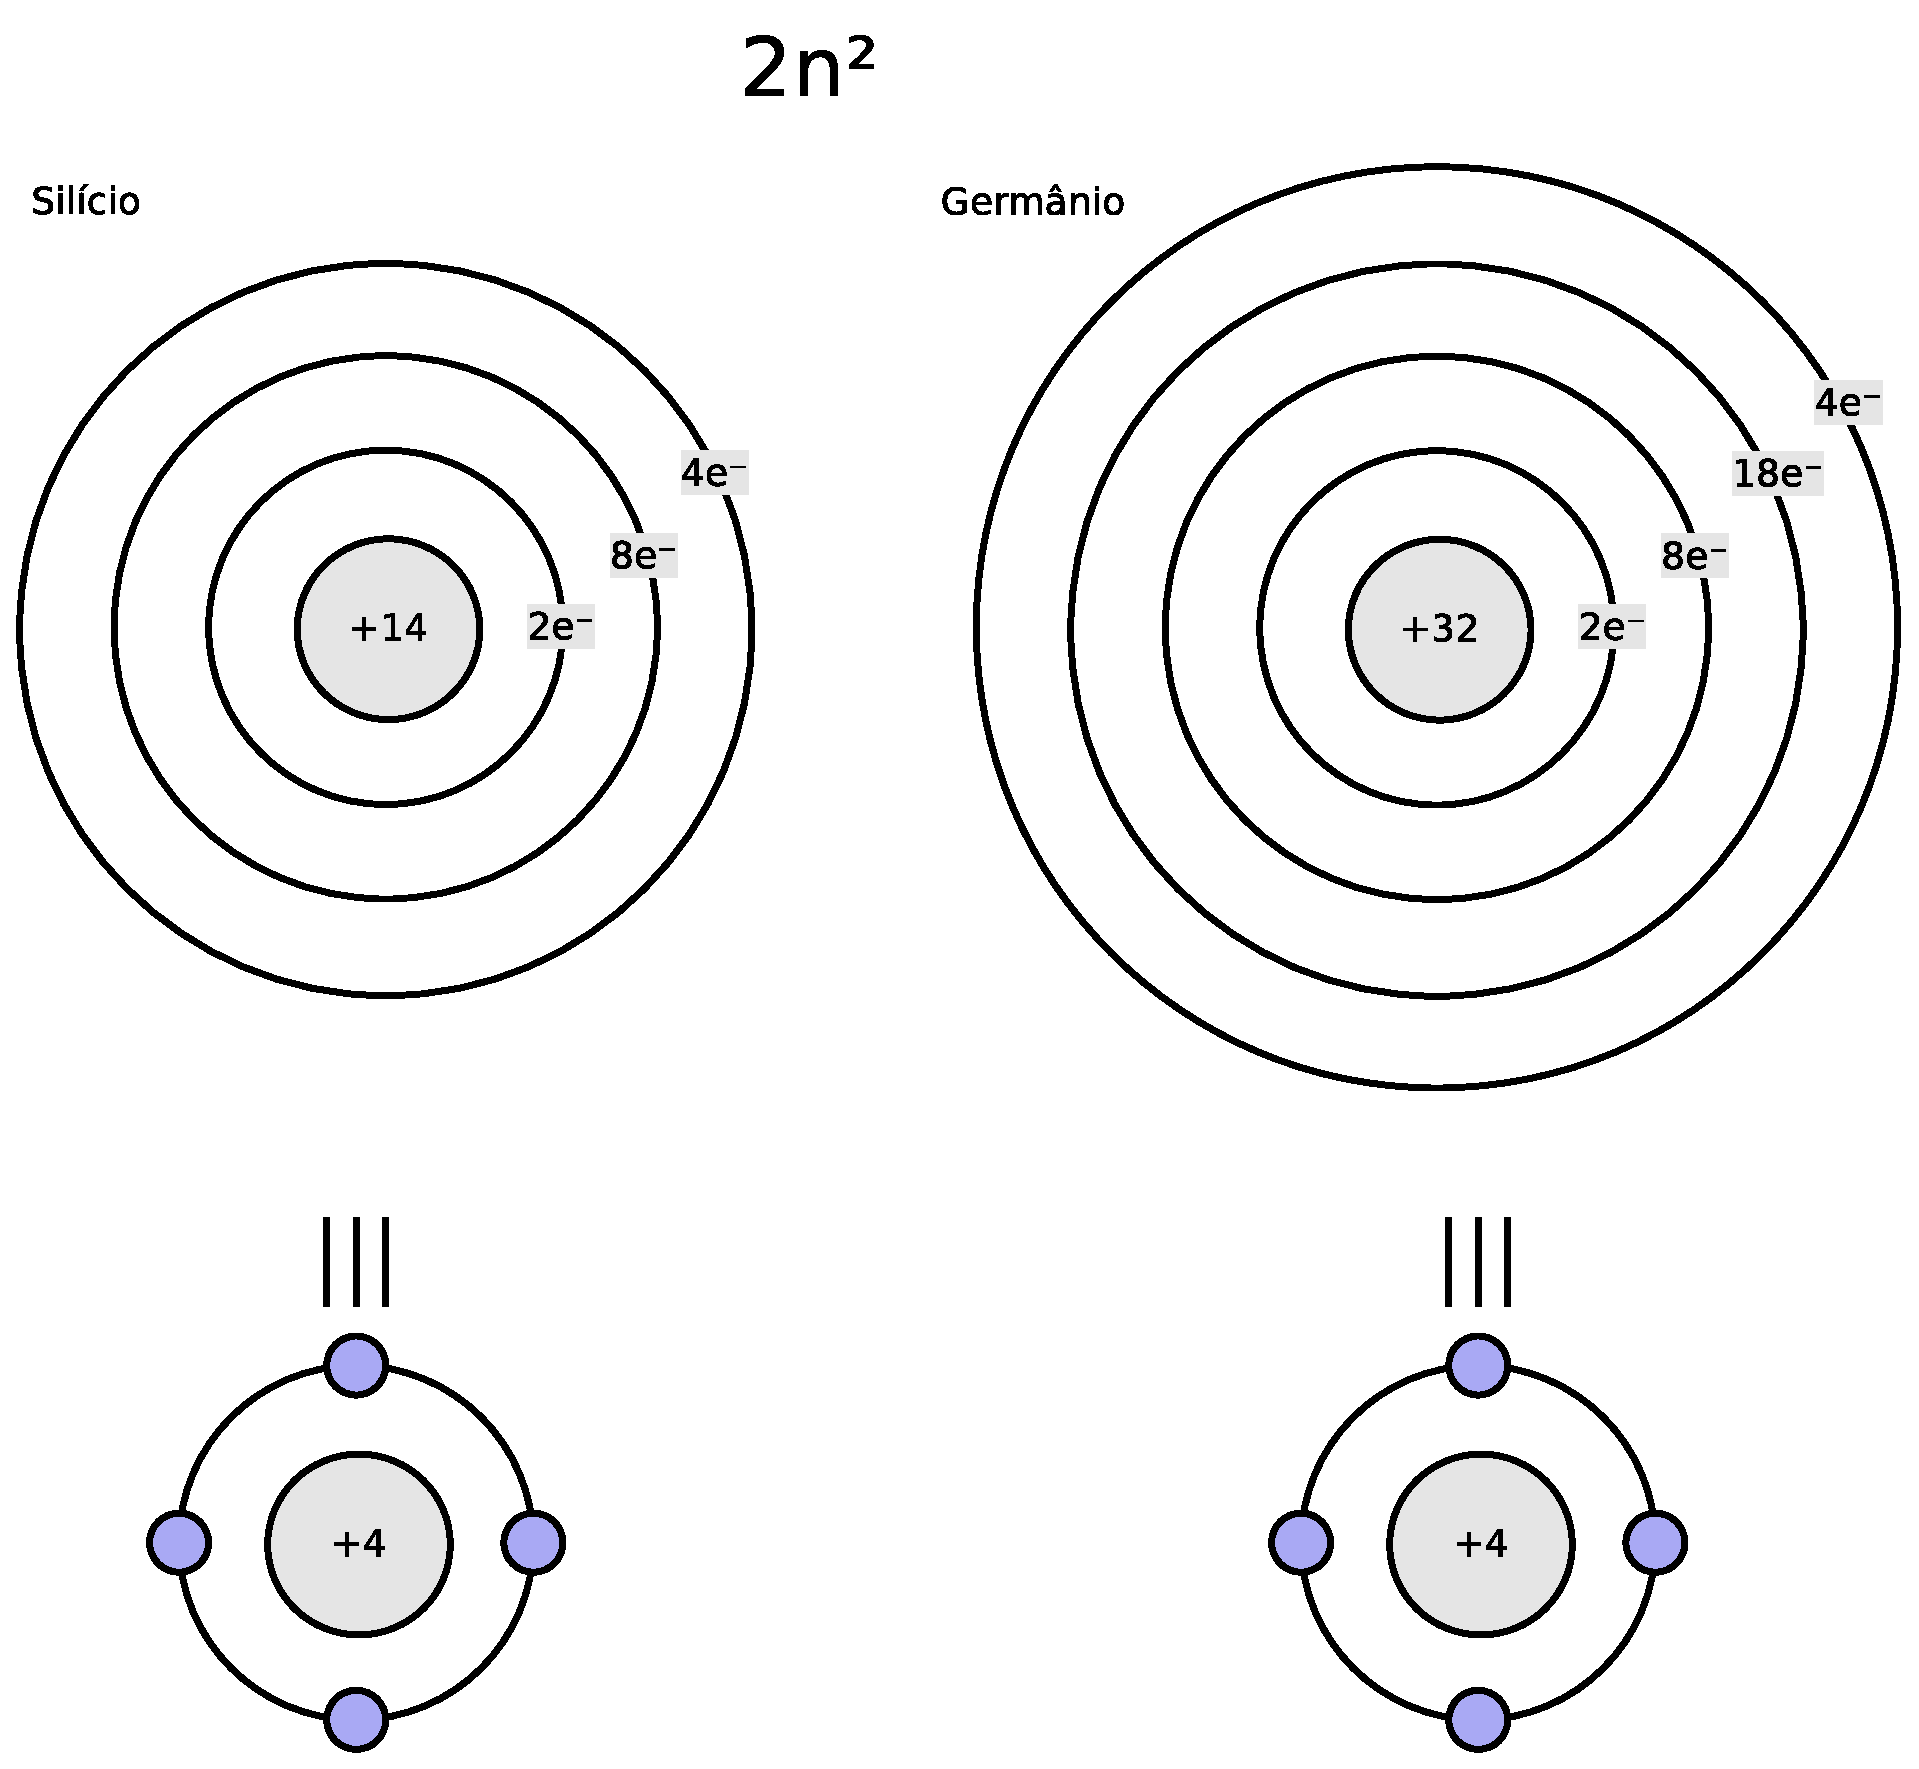
\includegraphics[width=5cm]{images/sige.eps}
\caption{Elétrons nas camadas e camadas de valência}
\label{fig:sige}
\end{figure}
\end{frame}

\begin{frame}{Semicondutor intrínseco}
\begin{figure}
\centering
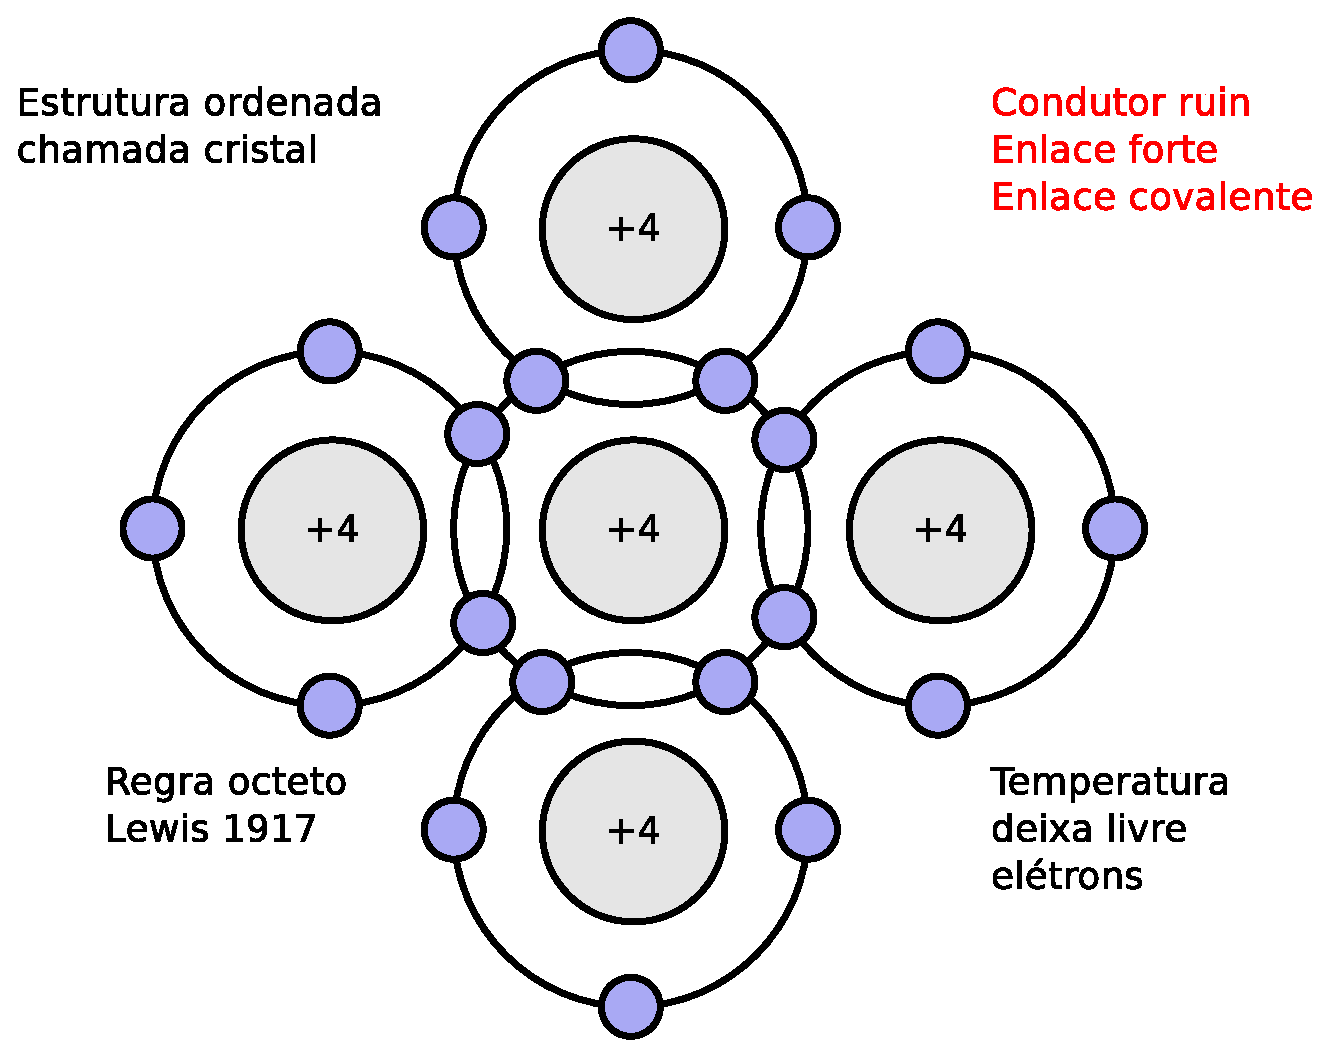
\includegraphics[width=6cm]{images/covalente.eps}
\caption{Semicondutor intrínseco (Semicondutor Puro)}
\label{fig:sige}
\end{figure}
\end{frame}

\begin{frame}{Dopagem: Semicondutor extrínseco tipo P}
\begin{figure}
\centering
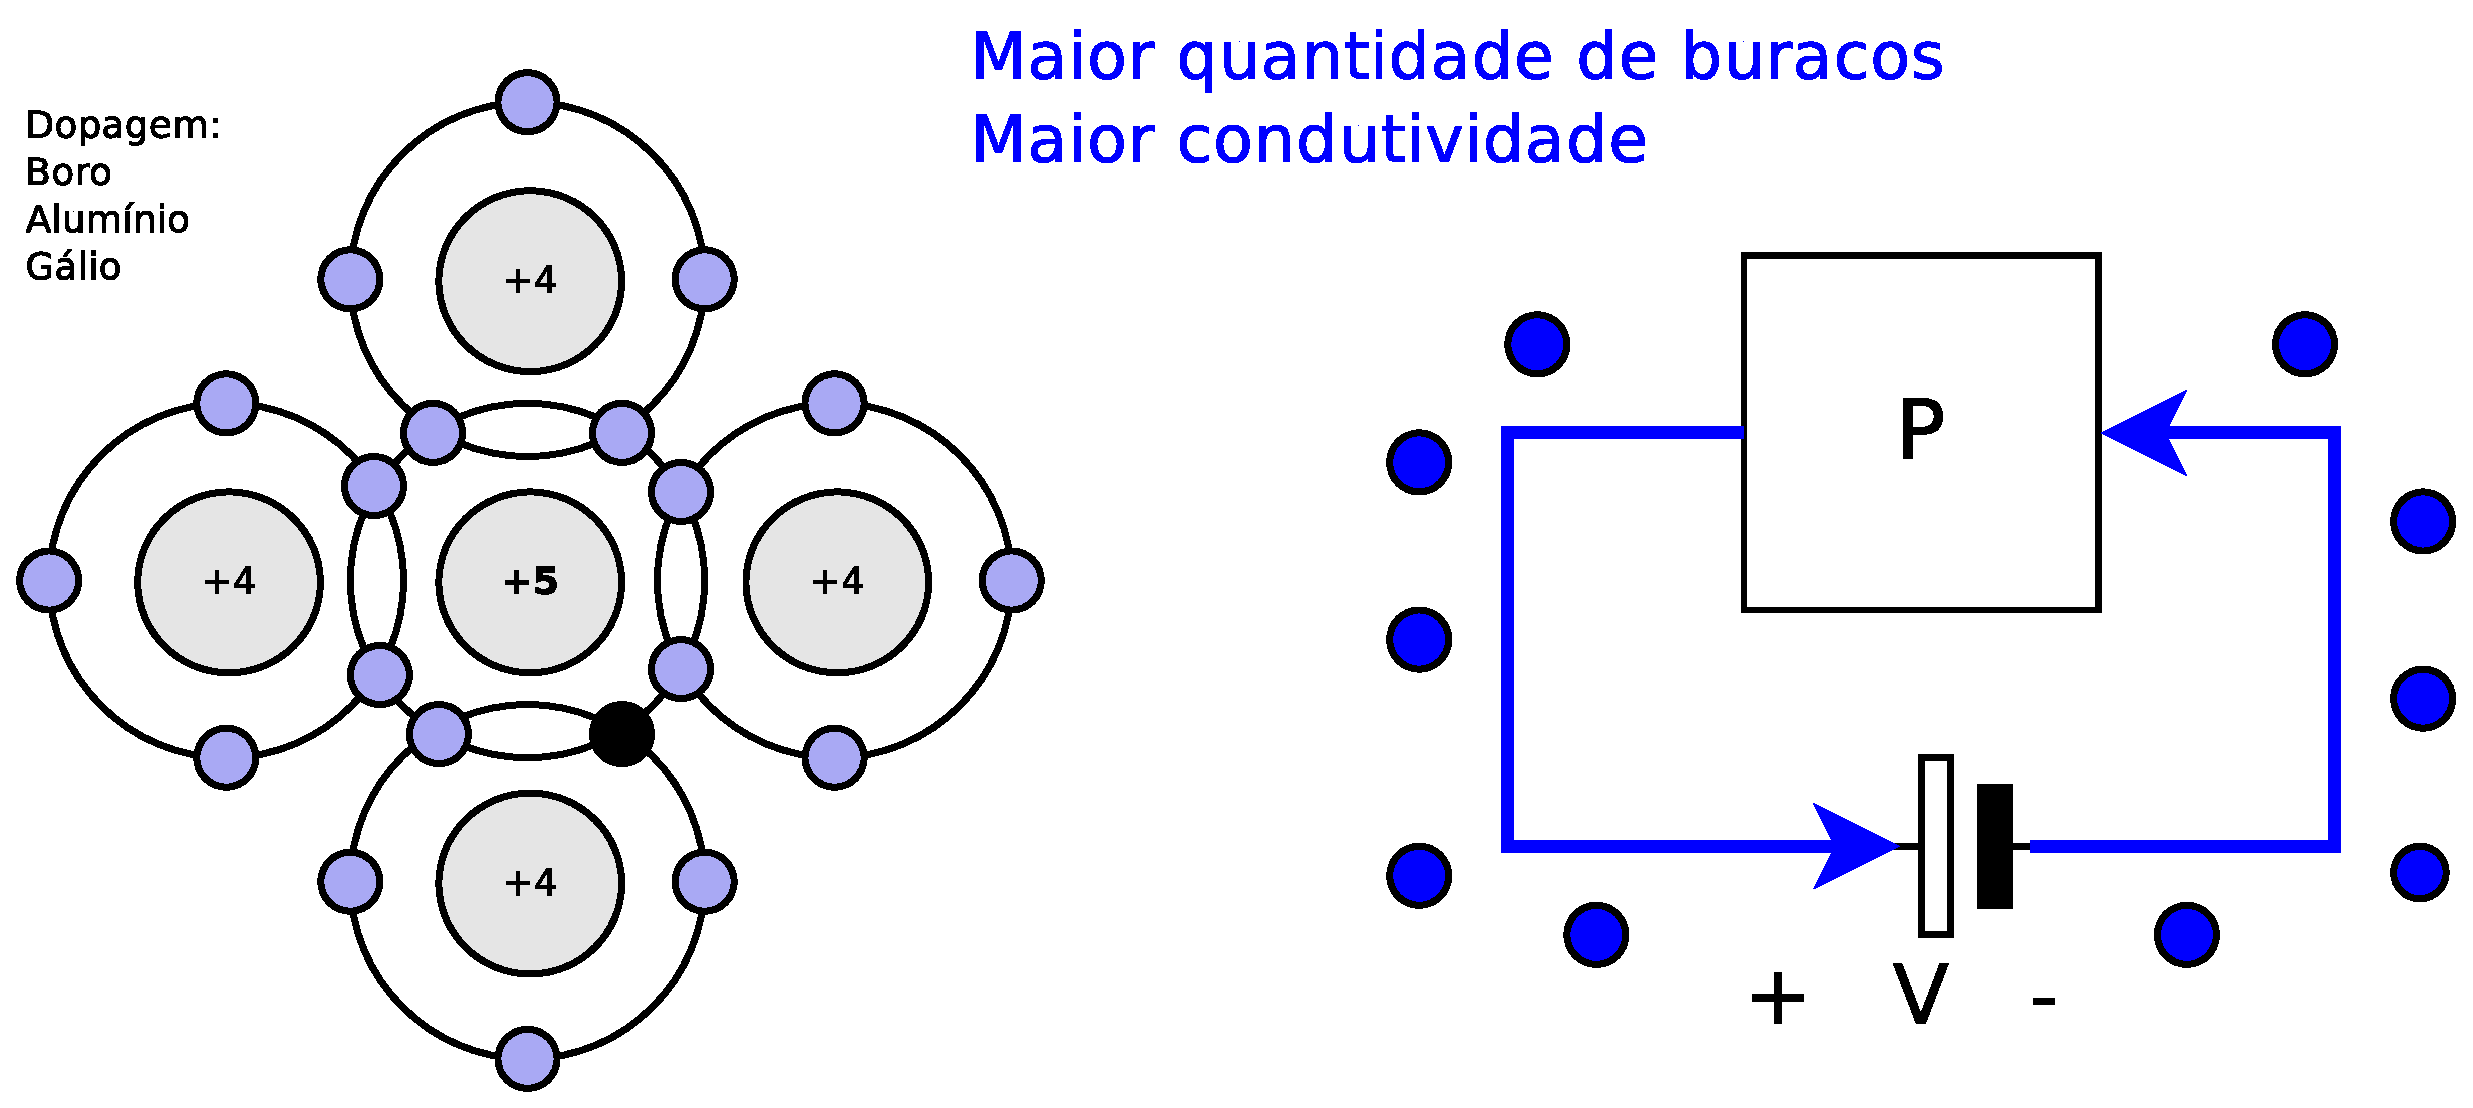
\includegraphics[width=10cm]{images/extrinsecop.eps}
\caption{Semicondutor extrínseco tipo P}
\label{fig:semip}
\end{figure}
\end{frame}

\begin{frame}{Dopagem:Semicondutor extrínseco tipo N}
\begin{figure}
\centering
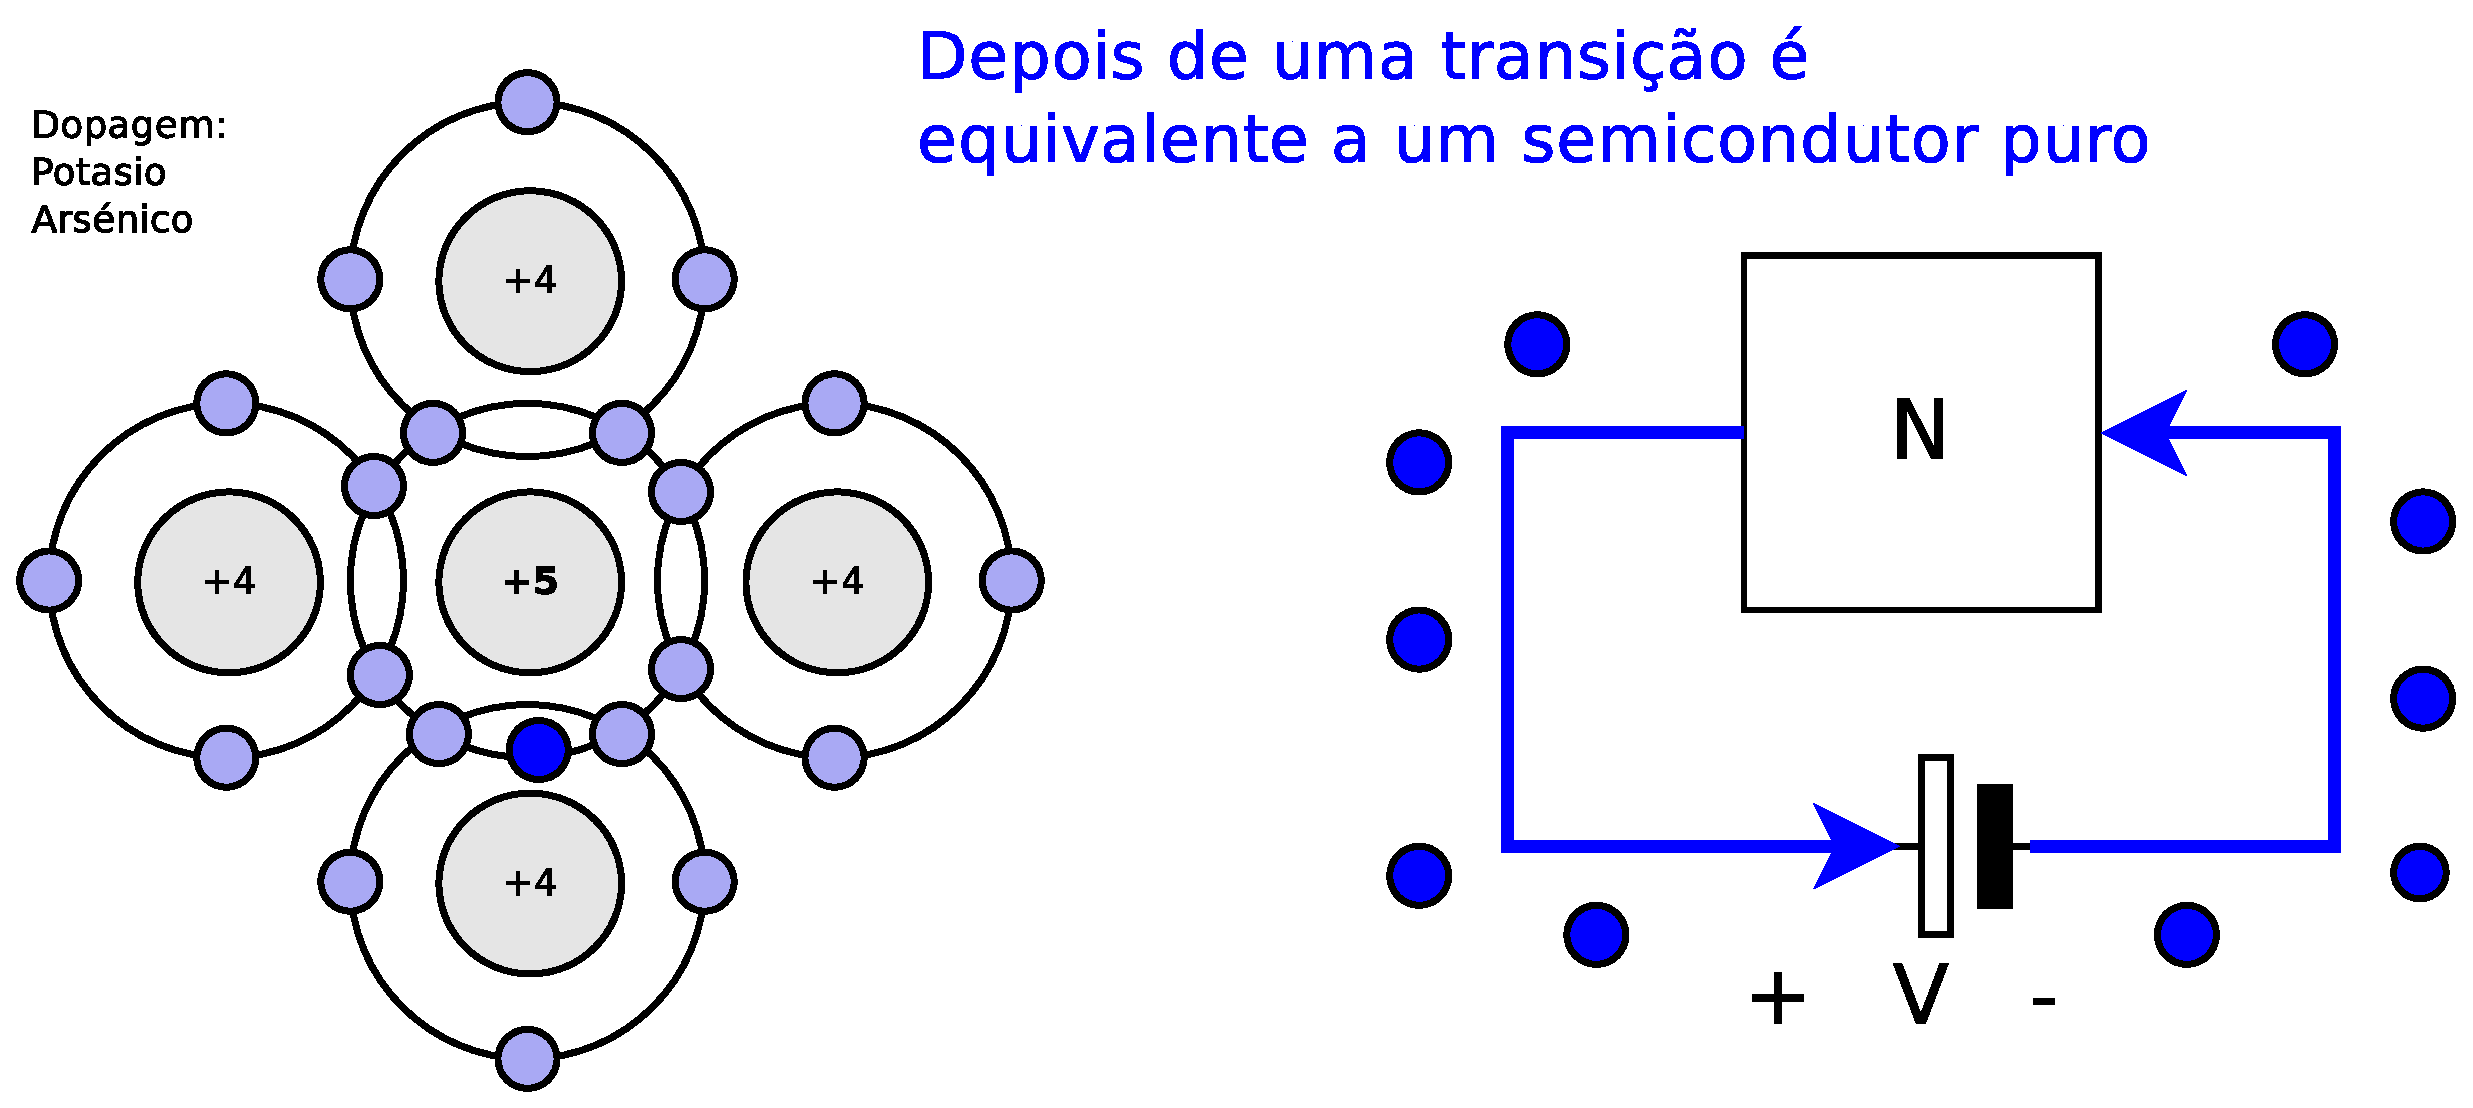
\includegraphics[width=10cm]{images/extrinsecon.eps}
\caption{Semicondutor extrínseco tipo N}
\label{fig:semin}
\end{figure}
\end{frame}

\begin{frame}{União PN  }
\begin{figure}
\centering
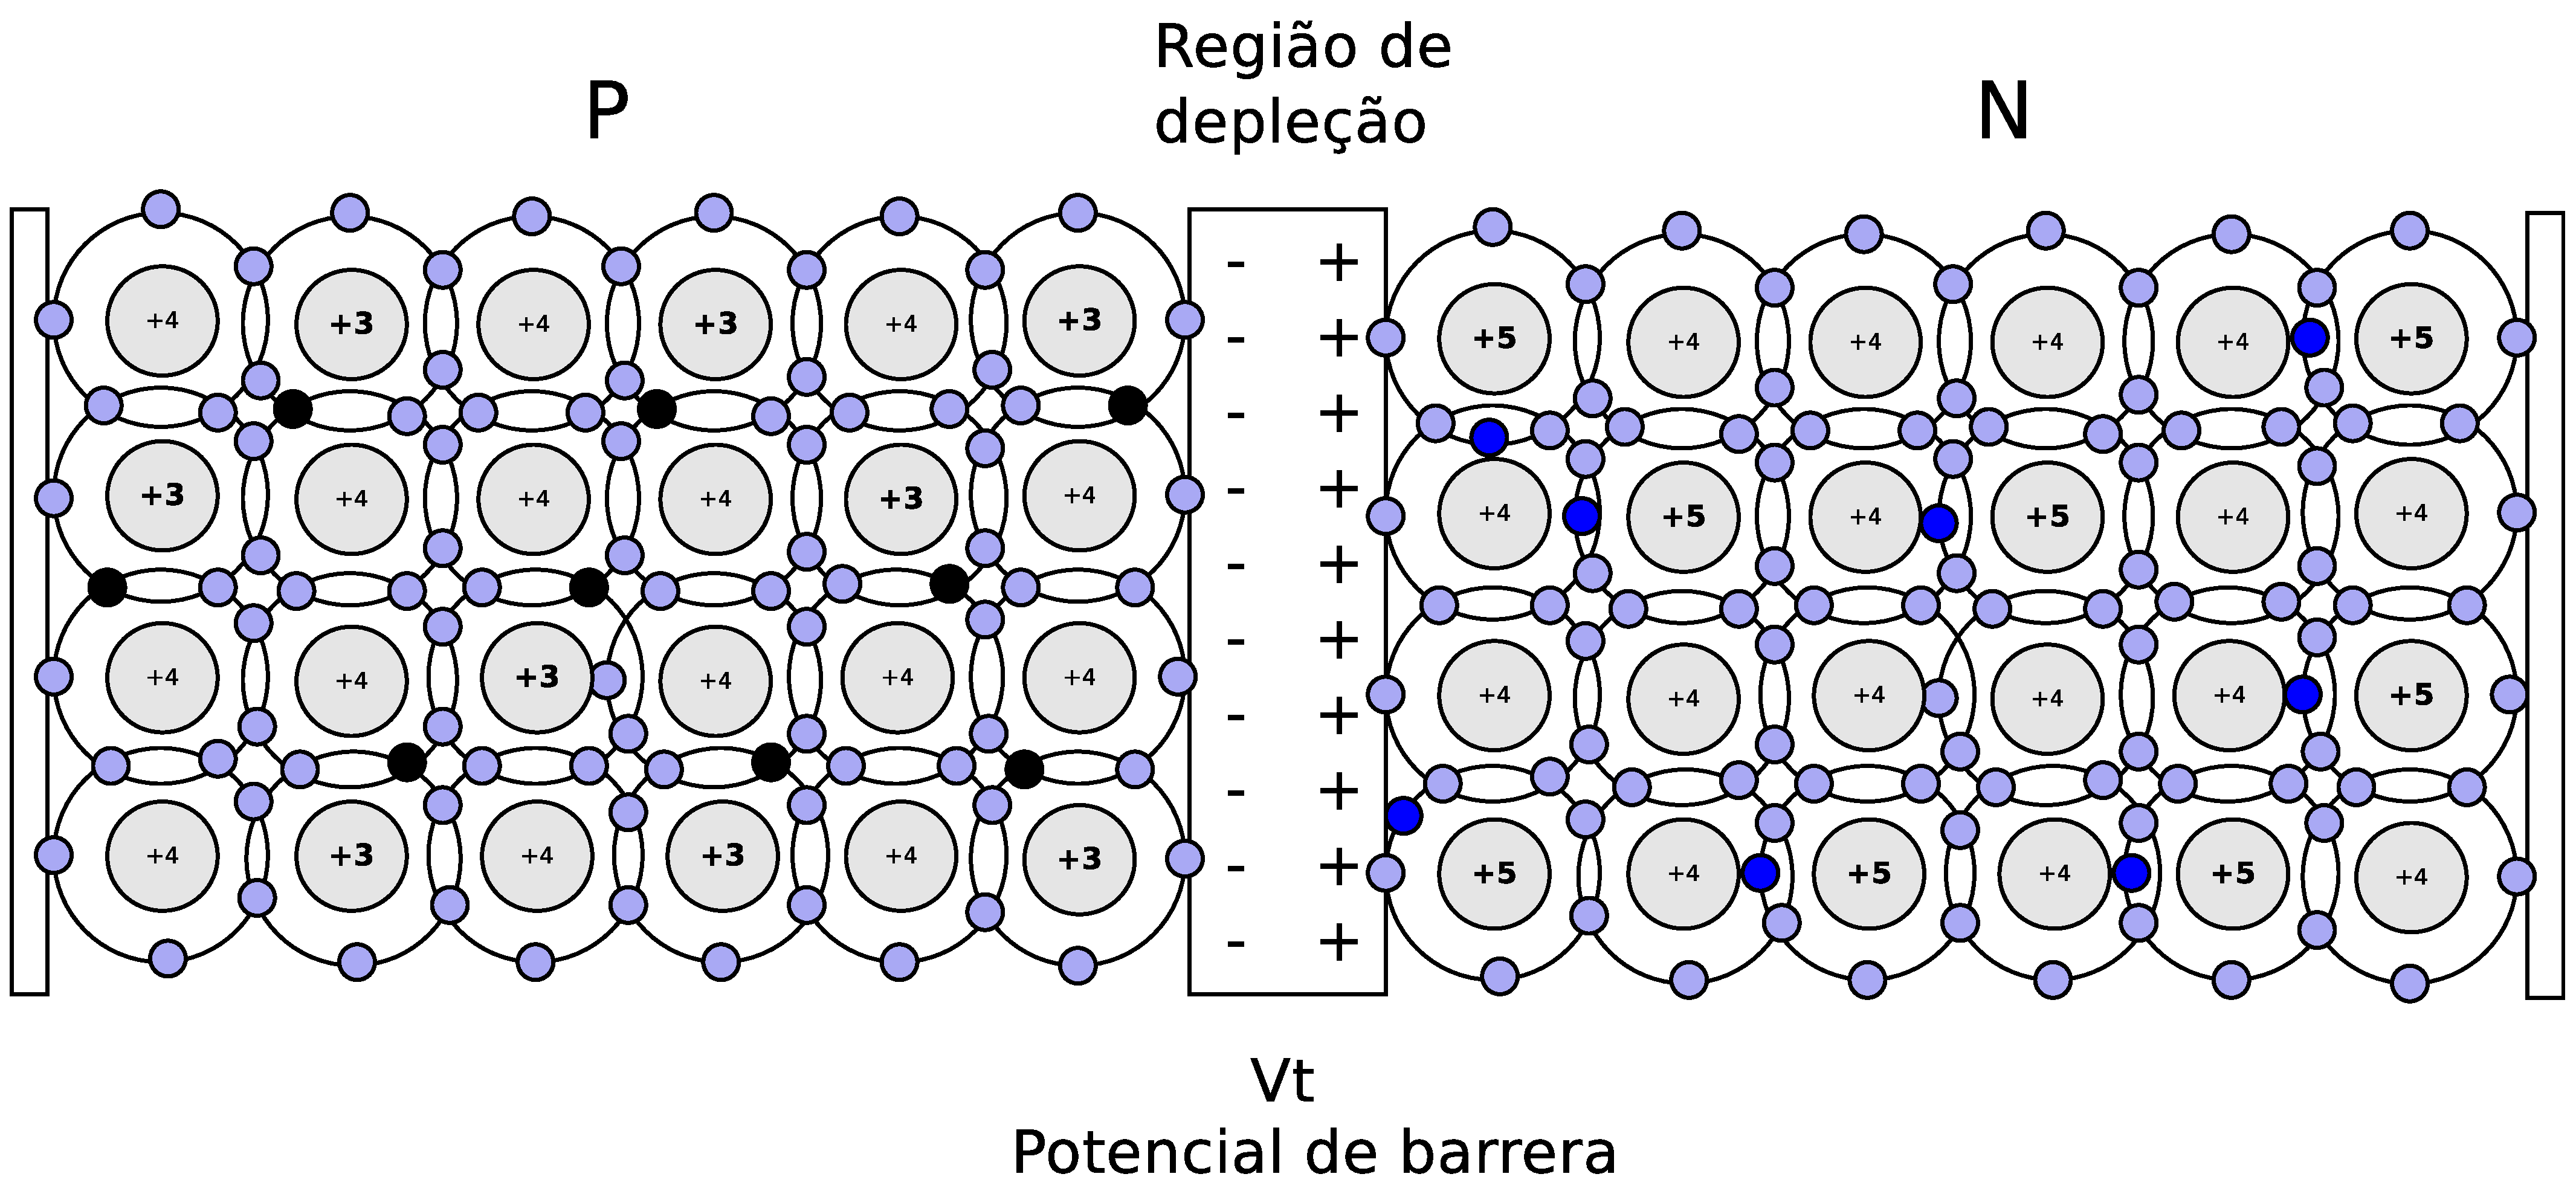
\includegraphics[width=9cm]{images/semipn0.eps}
\caption{Anodo - catodo}
\label{fig:semipn0}
\end{figure}
\end{frame}

\begin{frame}{União PN - Polarização direta }
\begin{figure}
\centering
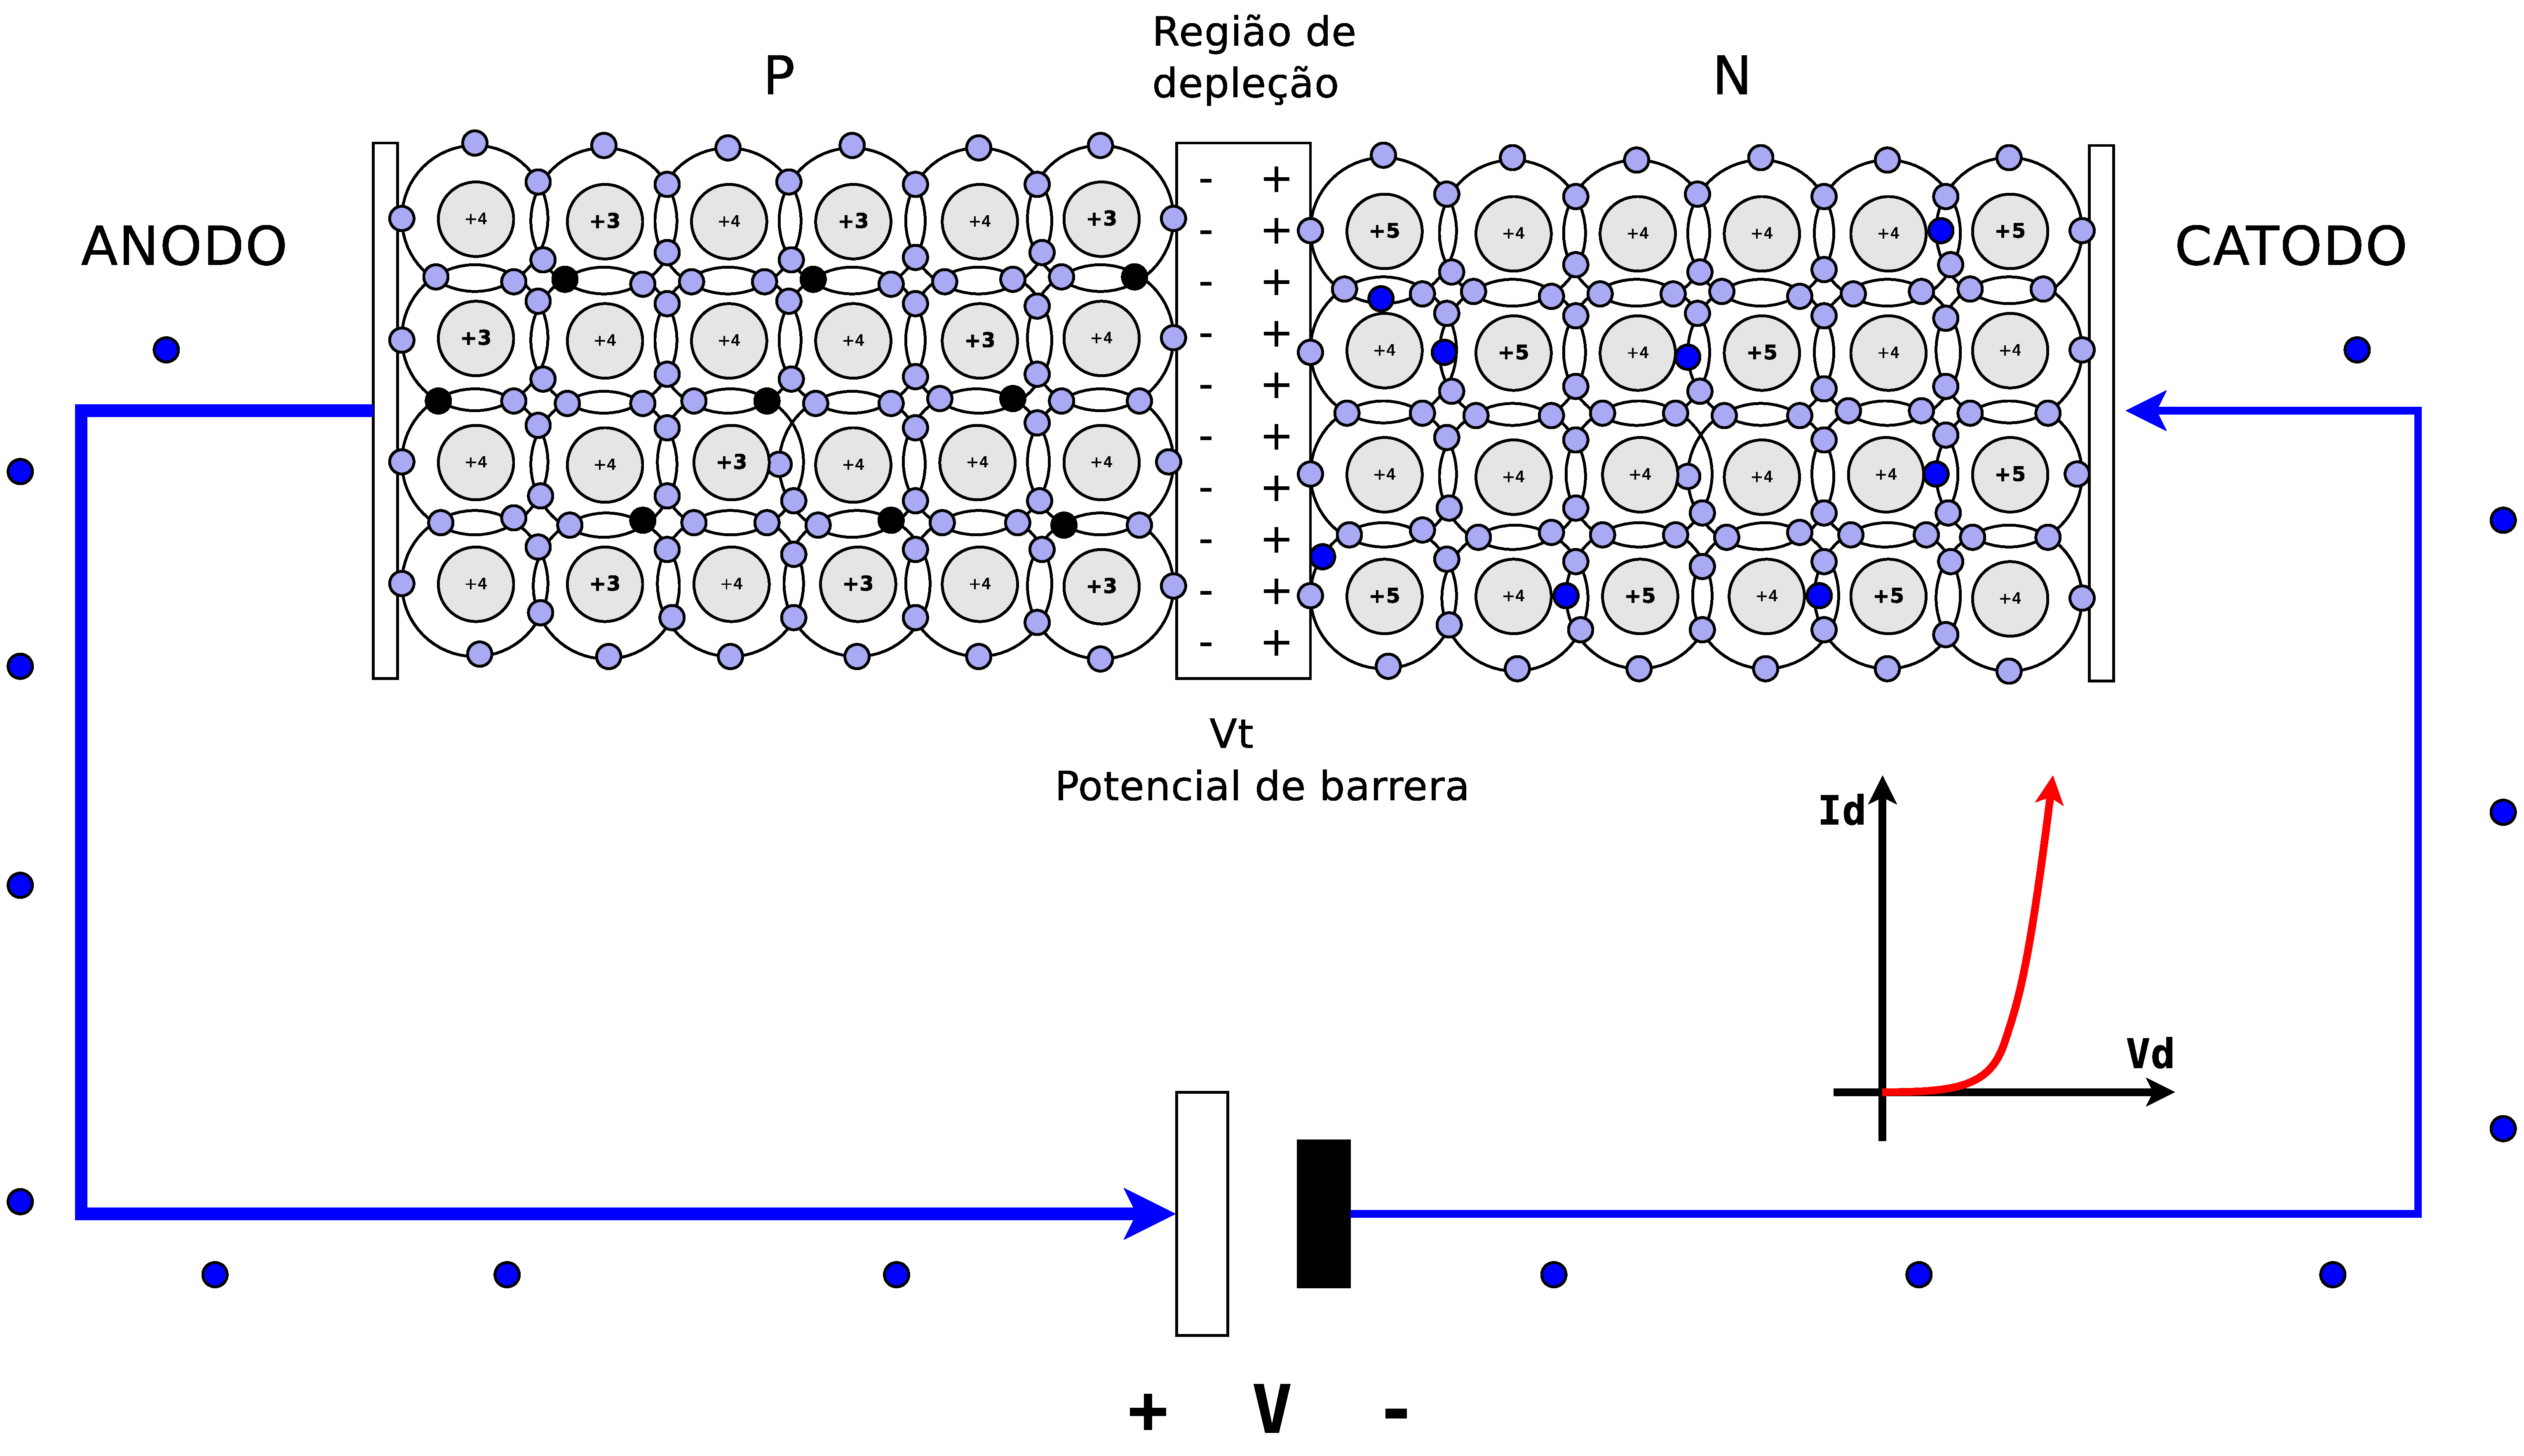
\includegraphics[width=9cm]{images/semipn.eps}
\caption{Polarização direta}
\label{fig:semipn0}
\end{figure}
\end{frame}

\begin{frame}{União PN - Polarização inversa }
\begin{figure}
\centering
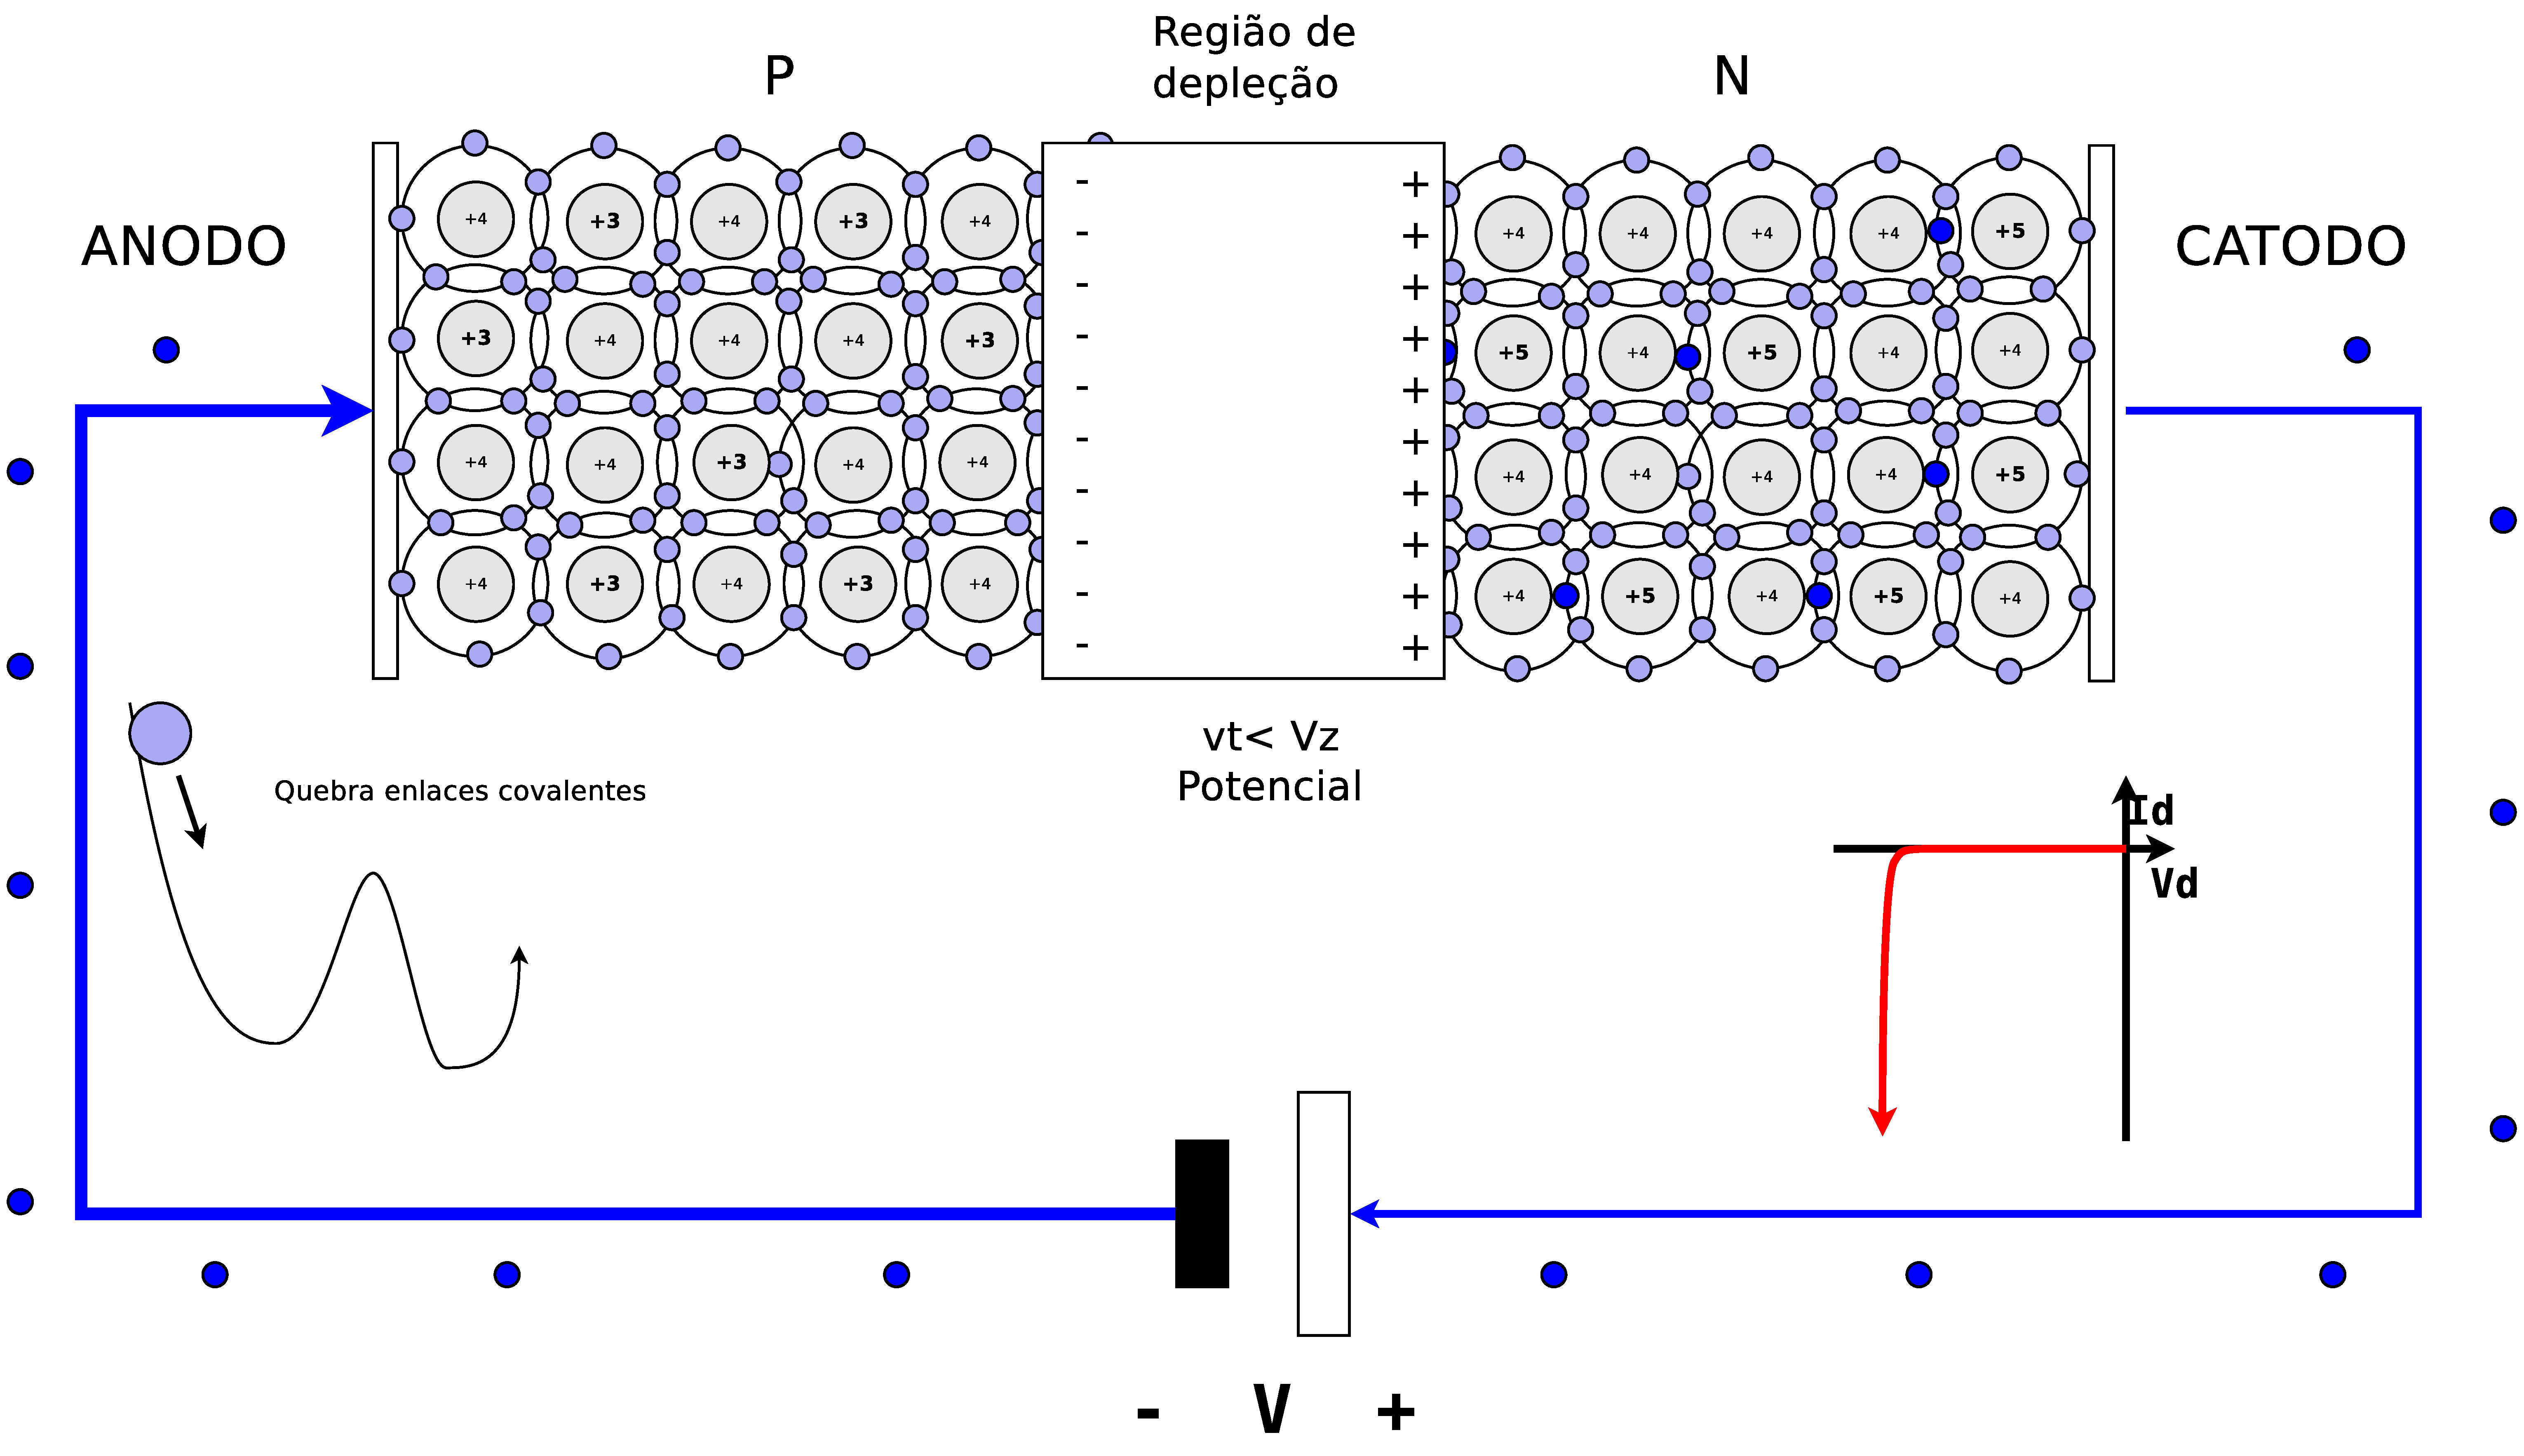
\includegraphics[width=9cm]{images/semipn2.eps}
\caption{Polarização inversa}
\label{fig:semipn0}
\end{figure}
\end{frame}

%%%%%%%%%%%%%%%%%%%%%%%%%%%%%%%%%%%%%%%%%%%%%%%%%%%%%%%%%%%%%%%%%%%%%%%%%%%%%%%%
%%%%%%%%%%%%%%%%%%%%%%%%%%%%%%%%%%%%%%%%%%%%%%%%%%%%%%%%%%%%%%%%%%%%%%%%%%%%%%%%
%%%%%%%%%%%%%%%%%%%%%%%%%%%%%%%%%%%%%%%%%%%%%%%%%%%%%%%%%%%%%%%%%%%%%%%%%%%%%%%%
\section{Caraterísticas}

\begin{frame}{Diodo  real}
\begin{figure}
\centering
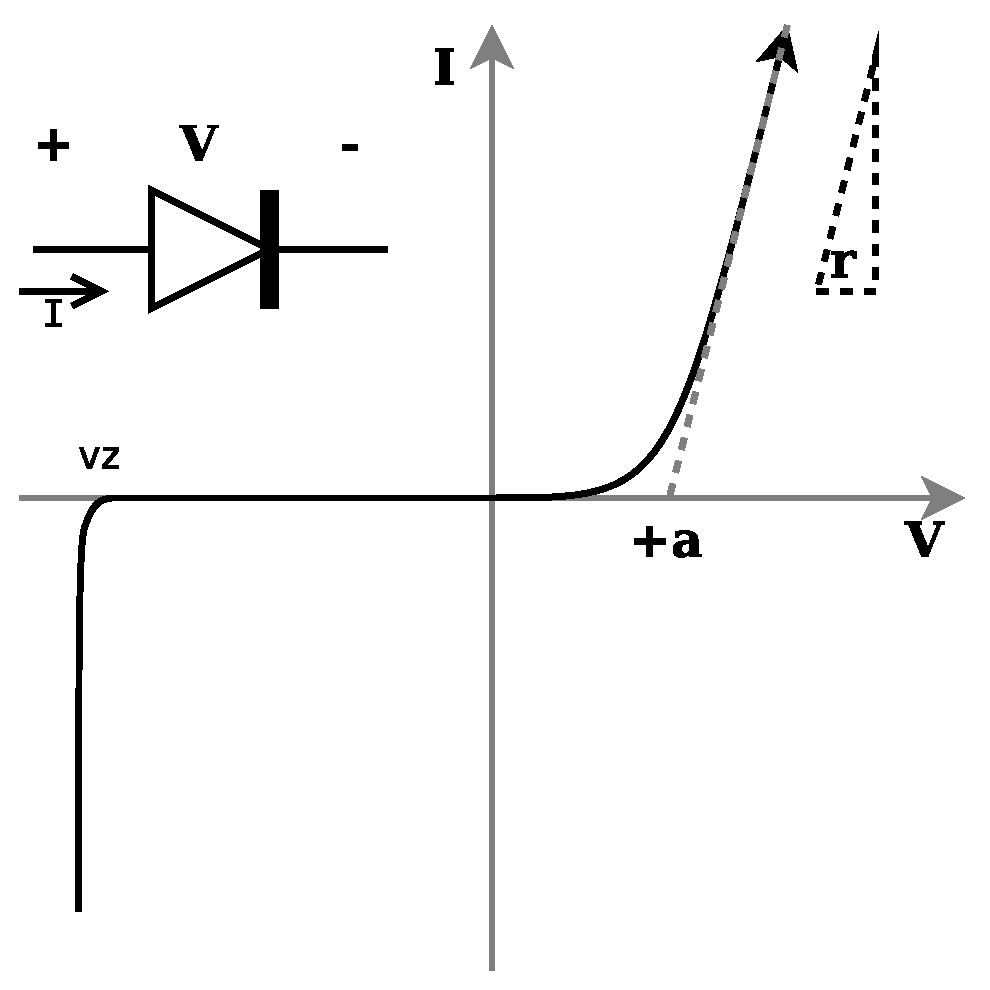
\includegraphics[width=5cm]{images/dreal.eps}
\caption{Diodo real -  Curva característica do diodo}
\label{fig:dreal}
\end{figure}
\end{frame}

\begin{frame}{Diodo  real}
\begin{figure}
\centering
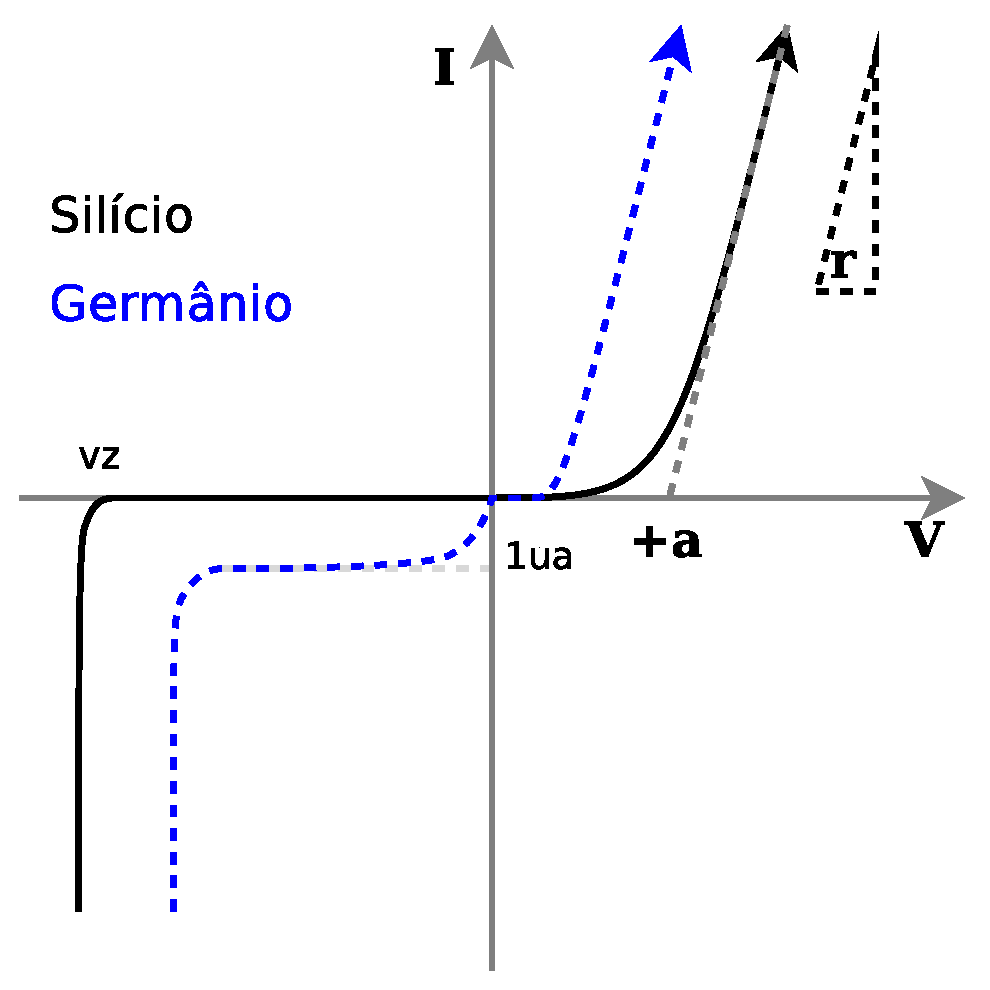
\includegraphics[width=6cm]{images/dreal2.eps}
\caption{Polarização direta -  Curva característica do diodo}
\label{fig:dreal}
\end{figure}
\end{frame}

\begin{frame}{Resistência no diodo}
\begin{figure}
\centering
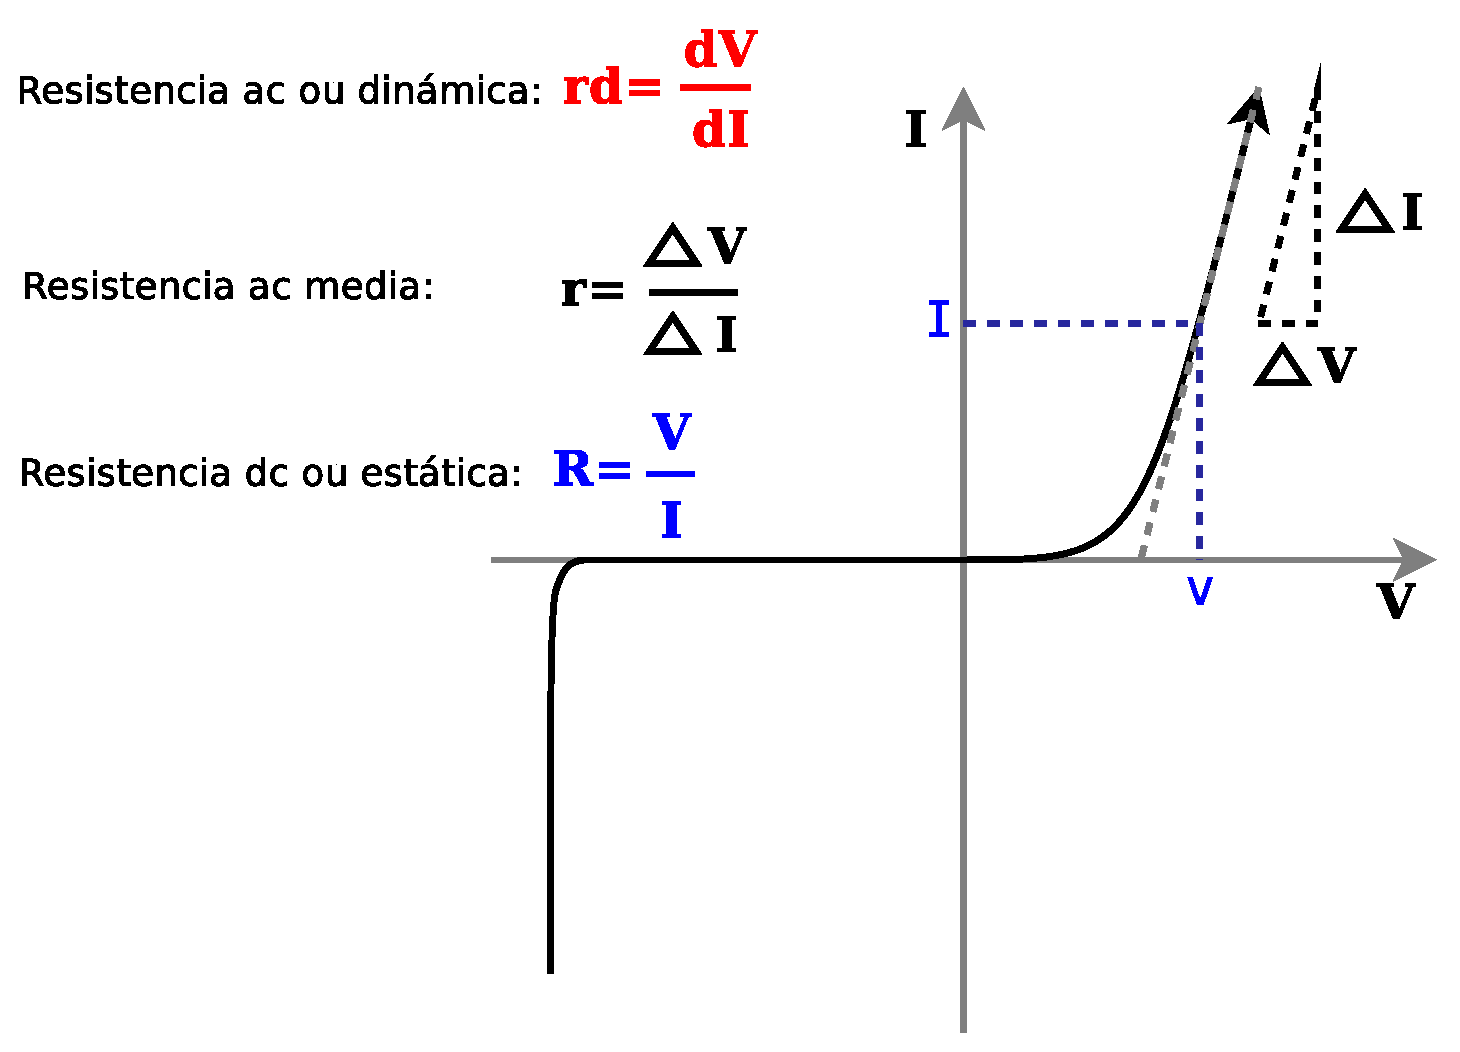
\includegraphics[width=7cm]{images/resaverdia.eps}
\caption{Diodo real -  Curva característica do diodo}
\label{fig:resaverdia}
\end{figure}
\end{frame}

\begin{frame}{Diodo  ideal e circuito equivalente de diodo}
\begin{figure}
\centering
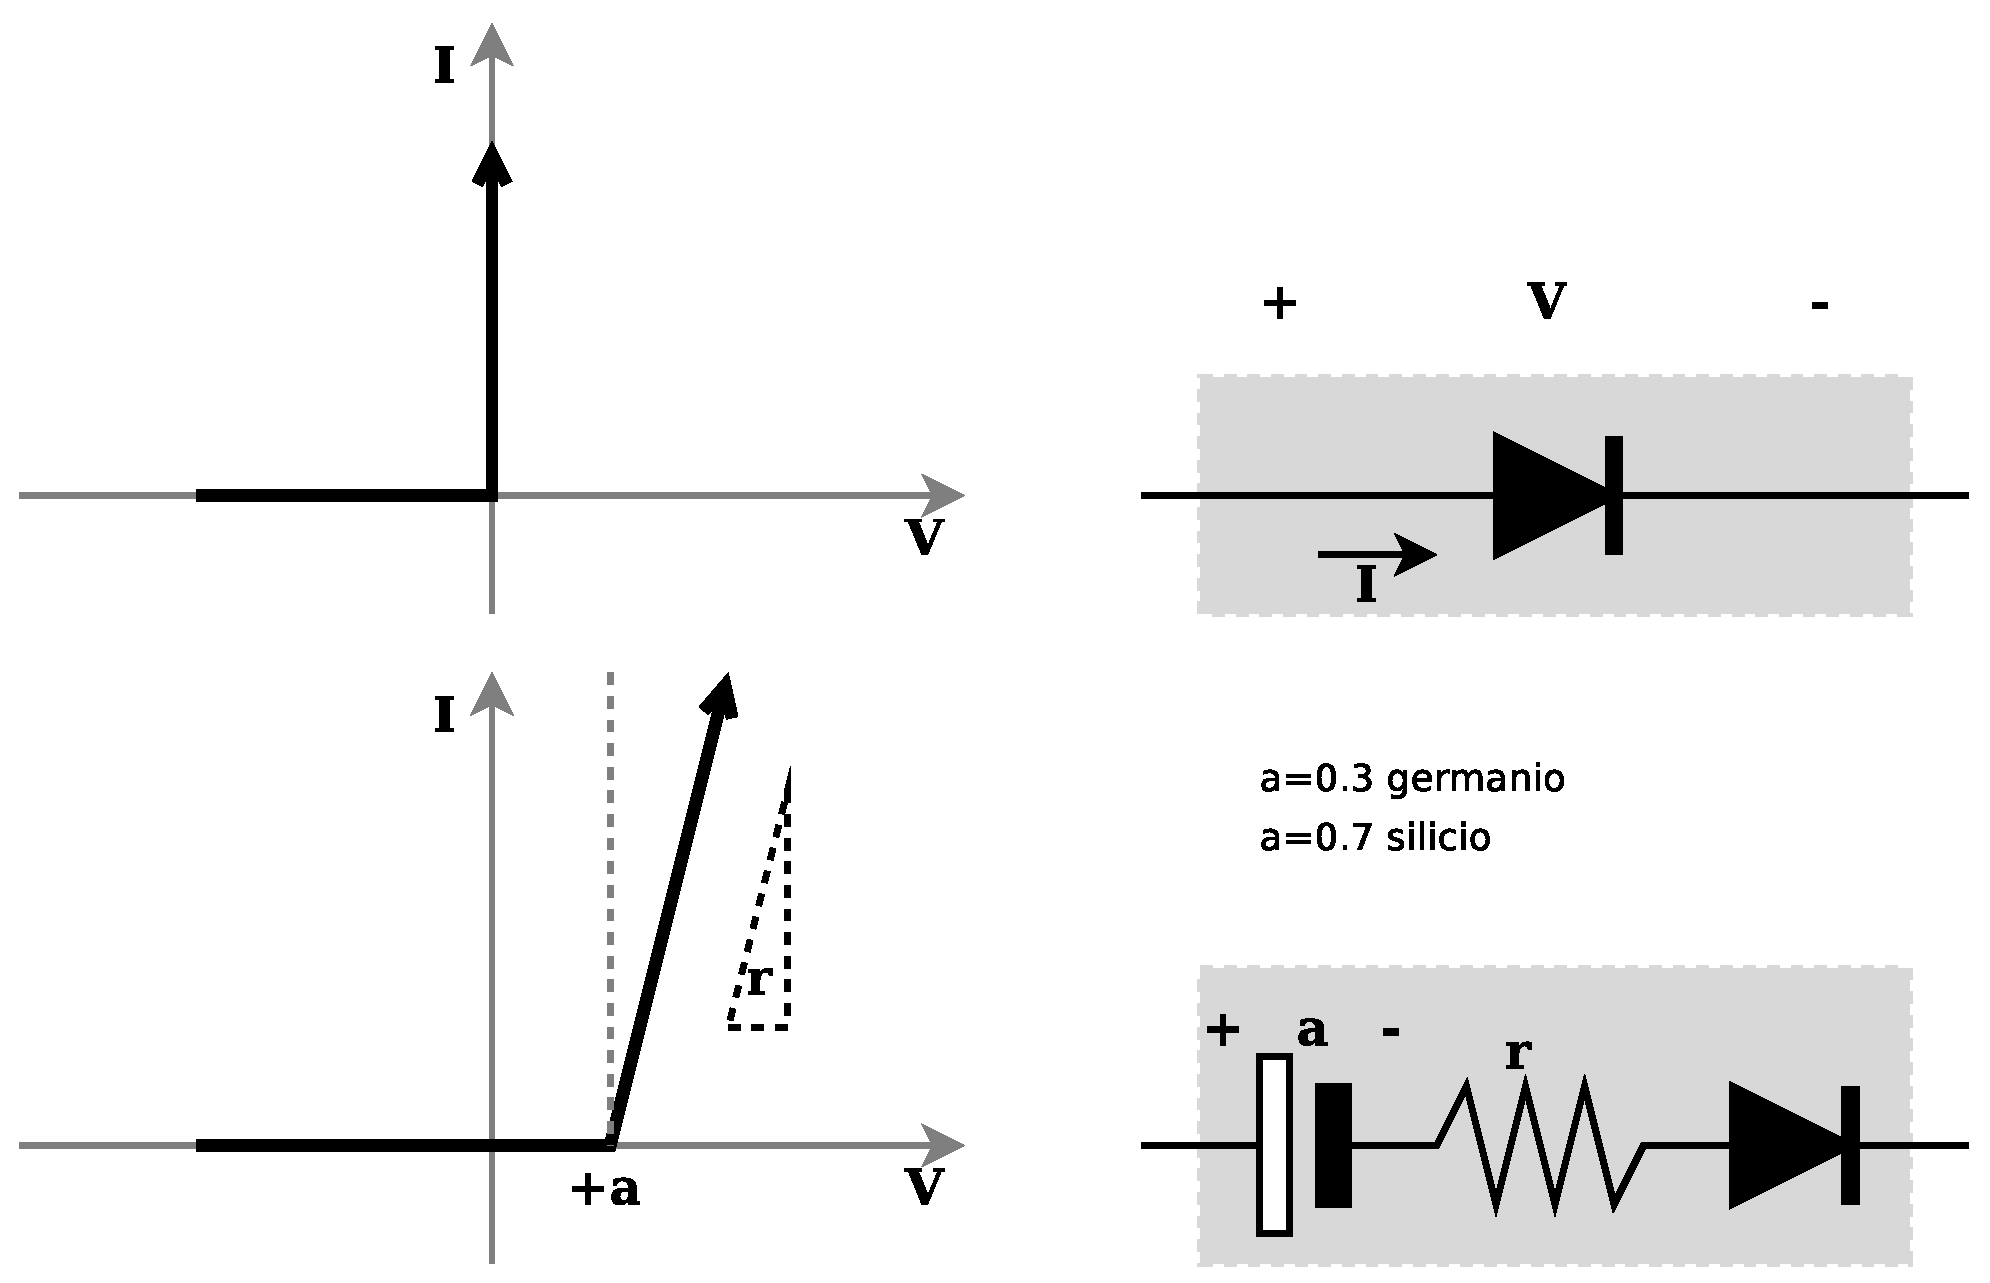
\includegraphics[width=8cm]{images/ideal.eps}
\caption{Diodo ideal e circuito equivalente de diodo}
\label{fig:ideal}
\end{figure}
\end{frame}

%%%%%%%%%%%%%%%%%%%%%%%%%%%%%%%%%%%%%%%%%%%%%%%%%%%%%%%%%%%%%%%%%%%%%%%%%%%%%%%%
%%%%%%%%%%%%%%%%%%%%%%%%%%%%%%%%%%%%%%%%%%%%%%%%%%%%%%%%%%%%%%%%%%%%%%%%%%%%%%%%
%%%%%%%%%%%%%%%%%%%%%%%%%%%%%%%%%%%%%%%%%%%%%%%%%%%%%%%%%%%%%%%%%%%%%%%%%%%%%%%%
\section{Aplicações}
\begin{frame}{Retificador de fonte: De meia onda}
\begin{figure}
\centering
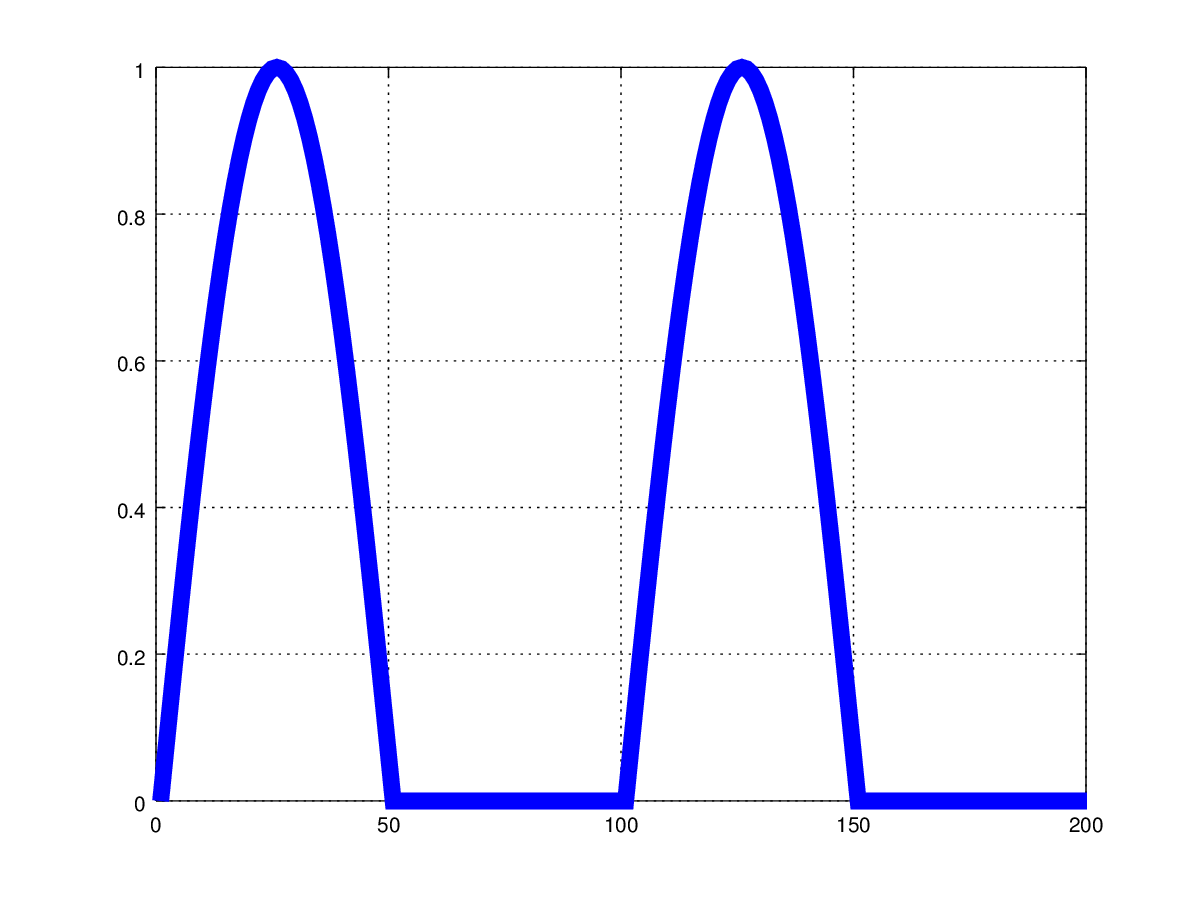
\includegraphics[width=5cm]{images/meiaonda.eps}
\caption{Deixa passar a corrente elétrica num sentido }
\label{fig:meiaonda}
\end{figure}
\end{frame}

\begin{frame}{Retificador de fonte: De onda completa}
\begin{figure}
\centering
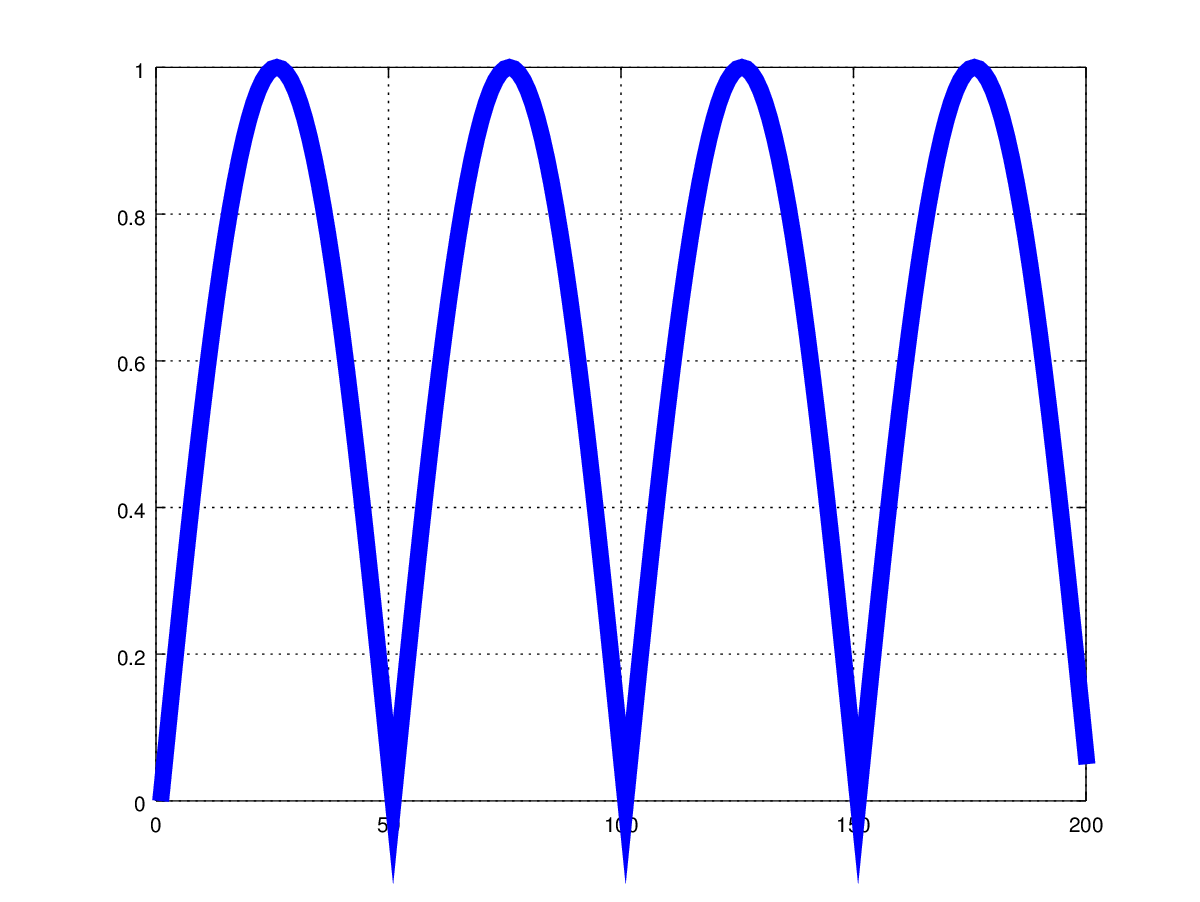
\includegraphics[width=5cm]{images/ondacompleta.eps}
\caption{Deixa passar a corrente uma vez por rama }
\label{fig:ondacompleta}
\end{figure}
\end{frame}

\begin{frame}{Retificador de fonte: De onda completa}
\begin{figure}
\centering
\includegraphics[width=8cm]{images/ponte.eps}
\caption{Deixa passar a corrente uma vez por rama }
\label{fig:ponte}
\end{figure}
\end{frame}

\begin{frame}{Retificador de fonte: De onda completa}
\begin{figure}
\centering
\includegraphics[width=8cm]{images/ponte2.eps}
\caption{Deixa passar a corrente uma vez por rama }
\label{fig:ponte2}
\end{figure}
\end{frame}

%%%%%%%%%%%%%%%%%%%%%%%%%%%%%%%%%%%%%%%%%%%%%%%%%%%%%%%%%%%%%%%%%%%%%%%%%%%%%%%%
\begin{frame}[allowframebreaks]
        \frametitle{References}
        \bibliographystyle{plain}
\bibliography{diodos}
\end{frame}



\end{document}
